\documentclass[main.tex]{subfiles}
\begin{document}

\chapter{Model}
\label{chapter:model}
% TODO Toto: verdient een introductie. waarom ga je het model in stages opbouwen? waarom wordt er een limiting factor gezien? 
% TODO Duidelijkere verwijzing naar problem statement. Een uitgewerkte problem statement is ook een goed idee.

This chapter will propose a model that provides a theoretical solution to the problem statement as described in section \ref{sectionproblemstatement}. This model addresses the problem statement from a technical and architectural point of view, as well as how user processes are affected. As a starting point, a description of a basic model for experiment setups on FPGA development boards is given in section \ref{sectionbasicmodel}, which is then extended and modified through a series of stages. In every stage, a particular aspect of the problem statement is addressed, forming a complete solution eventually. 

In section \ref{sectionvirtualizingio} the possible limiting factor of the  number of I/O devices on the FPGA development board is addressed by introducing the concept of a controller. This controller provides the experiment setup logic with a variable amount of virtual I/O channels. The levels of these I/O channels can then observed and controlled through controller-specific PC software. All of the physical I/O devices are temporarily removed from the model, as well as most of the FPGA's other peripheral devices.

In section \ref{sectioncyclecontrol} the controller is extended such that it allows for cycle-accurate control of sequential experiment setup logic. Users control cycles through the PC software, but the model supports autonomous operation as well. This new functionality is added through expansion of the experiment setup interface.

In section \ref{sectioncontrollerabstraction} the experiment controller's interface is generalized, such that the interface dependencies between experiment setup and controller are removed. This allows for independent development of controllers and experiment setups, allowing for random combinations of board-specific controllers and independent experiment setup logic. The controller's PC interface is generalized as well, which allows for the development of universal PC software.

% In section \ref{sectionreintroducingio} the FPGA development board's physical I/O devices are reintroduced into the model, after being removed from the model in section \ref{sectionvirtualizingio}. This step is essential in enabling a student's physical view of the experiment setup and providing a hands-on experience. The development of experiment setups remains an independent process.



\section{The Basic Model}
\label{sectionbasicmodel}

% TODO er worden een aantal zaken gepresenteerd waarvan een verwijzing ontbreekt. Hoewel er geen 1-1 verwijzing is in een aantal gevallen, kun je wel verwijzen naar de stukken op basis waarvan de gepresenteerde informatie is dedistileerd. 

% TODO in figuren en tekst onderscheid maken tussen I/O, HID, peripheral, communication device.

As a starting point, a description of a basic model for experiment setups on FPGA development boards is given. An overview of the basic model is displayed in figure \ref{fig:overview-basic}. The model features a PC and a FPGA development board as the two primary physical components. An interface between the PC and the FPGA development board exists over which the board exposes the \texttt{Board.Program()} operation. This operation initializes the FPGA by loading the contents of a FPGA-specific bitstream file and configuring the FPGA's components. The physical and electrical characteristics of this interface are considered to be irrelevant and may even be a process that involves manual user operations, such as transferring a memory card.


\begin{figure}[h]
    \centering
    \caption{The basic model, an overview of the FPGA development board and its exposed interfaces.}
    \label{fig:overview-basic}
    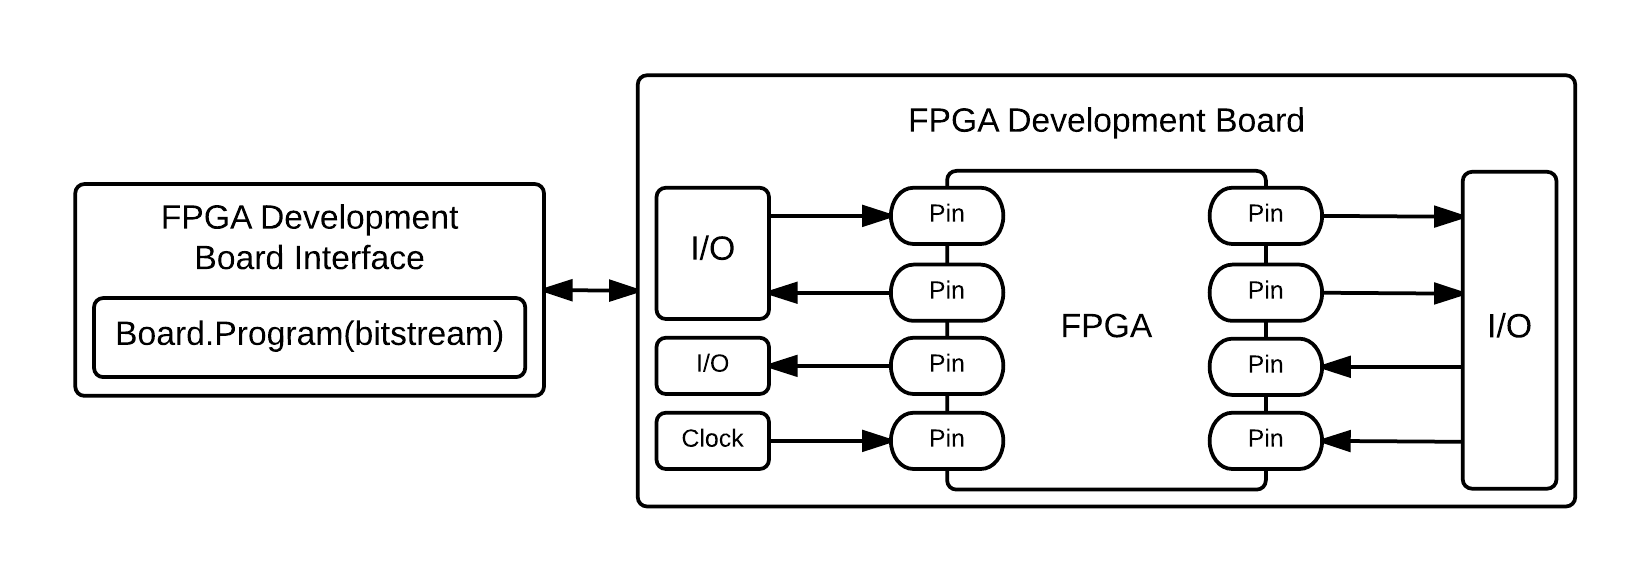
\includegraphics[width=0.8\textwidth]{img/overview-basic}
\end{figure}

In this basic model, the FPGA development board is considered to be a printed circuit board (PCB) which hosts and interconnects a FPGA and its various peripheral components. Not all pins of the FPGA package and not all peripheral devices are considered to be relevant to the model. Only the pins whose signals can be controlled through the FPGA's contained logic are included. Peripheral devices that do not connect to these pins, such as power supplies or programming circuits are excluded from the model. Specifically, the presence of a clock generating device is assumed, providing the FPGA with a clock signal on one of its pins. Although this model is a great simplification of reality, this abstract view is assumed to be sufficient for the purposes of this model and applicable to most FPGA development boards. 

Besides the omission of details of the FPGA's peripherals, a part of the FPGA's internal complexities are hidden from the model as well. Figure \ref{fig:fpga-basic} gives a graphical overview of the FPGA's internals and its contained logic. The FPGA's internal interface is simplified and defined to be a container for the end product of a HDL developer's work: an entity with input signals, output signals and an input clock signal. Other physical, electrical or logical characteristics of the FPGA are not included in the model.

\begin{figure}[h]
    \centering
    \caption{The basic model, an overview of the FPGA and its contained experiment setup logic. No specific architecture is applied to the logic.}
    \label{fig:fpga-basic}
    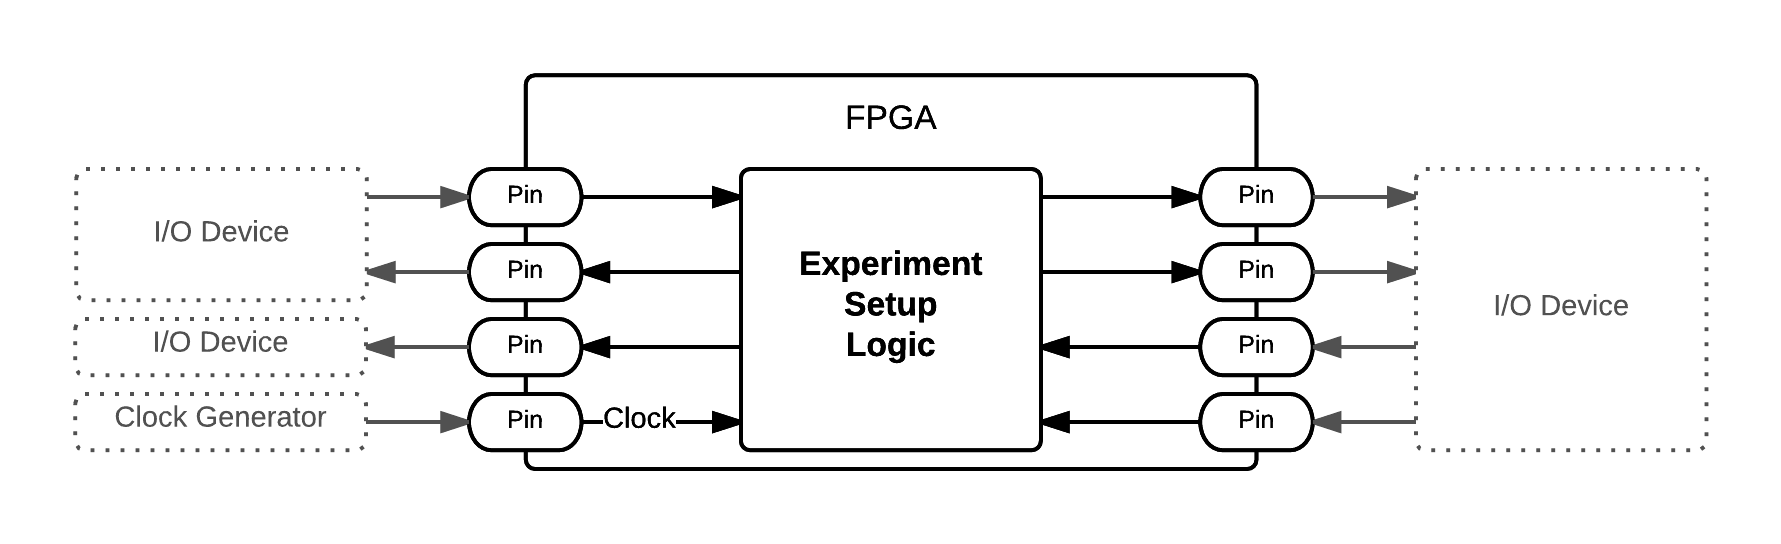
\includegraphics[width=\textwidth]{img/fpga-basic}
\end{figure}

In the case of this basic model, no specific architecture is defined that will embed the experiment setup logic into the FPGA development board. A specific architecture will be developed in the following stages. At this stage of the model, a developer is responsible for the development of its own architecture that embeds the experiment setup logic into the environment of the FPGA.

In this basic model, two user roles are defined: experiment setup developers and experimenters. In a classroom environment, an instructor can be considered an experiment setup developer and a student can be considered an experimenter. 

\subsection{Experiment Setup Developers}
\label{sectionexperimentdevelopers}
Experiment setup developers are responsible for the design, implementation, testing, documentation and distribution of experiment setups for use on FPGA development boards. The end product of their work is a software package that contains a bitstream file and optionally the source files used in the bitstream file's compilation process. Figure \ref{fig:process-development-basic} displays a graphical overview of the experiment setup development process. 

\begin{figure}[h]
    \centering
    \caption{The basic model, an overview of the experiment setup development process.}
    \label{fig:process-development-basic}
    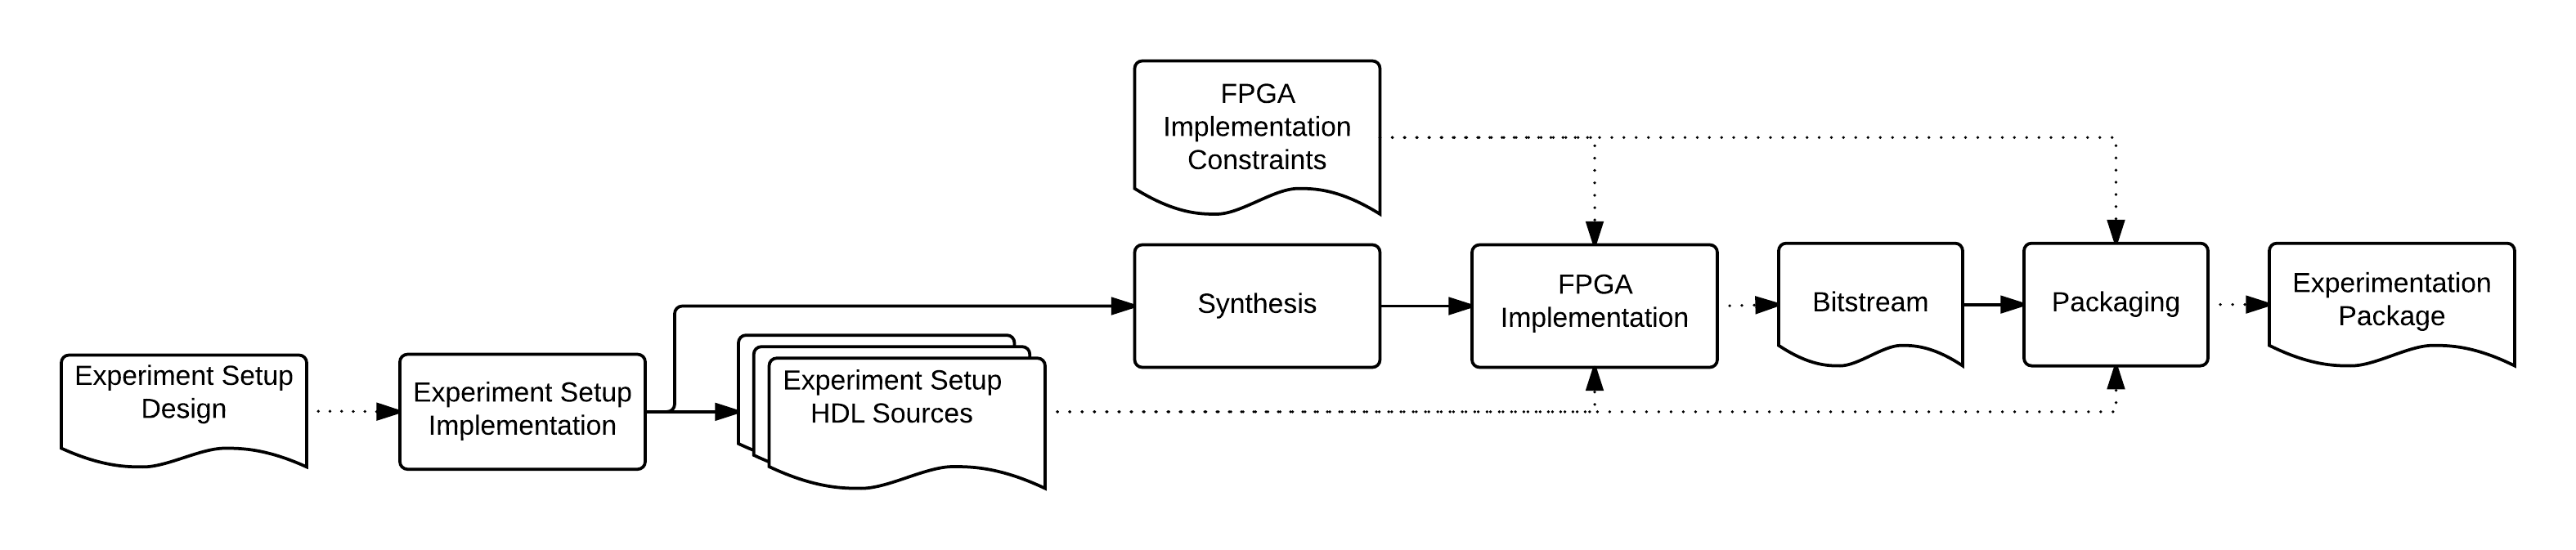
\includegraphics[width=\textwidth]{img/processes-basic-development}
\end{figure}


% TODO onderstaande opsomming is beter op zijn plaats in de problem statement.
As shown below, an experiment setup developer must have knowledge of a significant number of subjects and technologies: 

\begin{itemize}
\item Designing an experiment setup requires knowledge on the subject of digital logic and digital systems. 
\item For the design to contain meaningful educational content, the developer should have experience in teaching the subject. 
\item Translating the design into a working, valid implementation in VHDL or Verilog requires experience in HDL development.
\item Embedding the implemented design in a FPGA development board requires knowledge of the specific FPGA, its development tools and the FPGA's peripheral devices.
\end{itemize}

\subsection{Experimenters}

Experimenters are responsible for carrying out experiments. They obtain experiment setup software packages and initialize experiment setups on their FPGA development boards. In order to complete the experiment, they make observations and interact with the experiment setup that is contained within the FPGA. Figure \ref{fig:process-experimentation-basic} displays a graphical overview of the experimentation process. In this basic model, two different methods of interaction are defined: interaction through board I/O devices and interaction through the process of HDL source modification, recompilation and reprogramming. Observation of the experiment's results can be done through the FPGA development board's I/O devices. Some development tools allow for live inspection of the FPGA's internal signal levels through a PC connection.

\begin{figure}[h]
    \centering
    \caption{The basic model, an overview of the experimentation process.}
    \label{fig:process-experimentation-basic}
    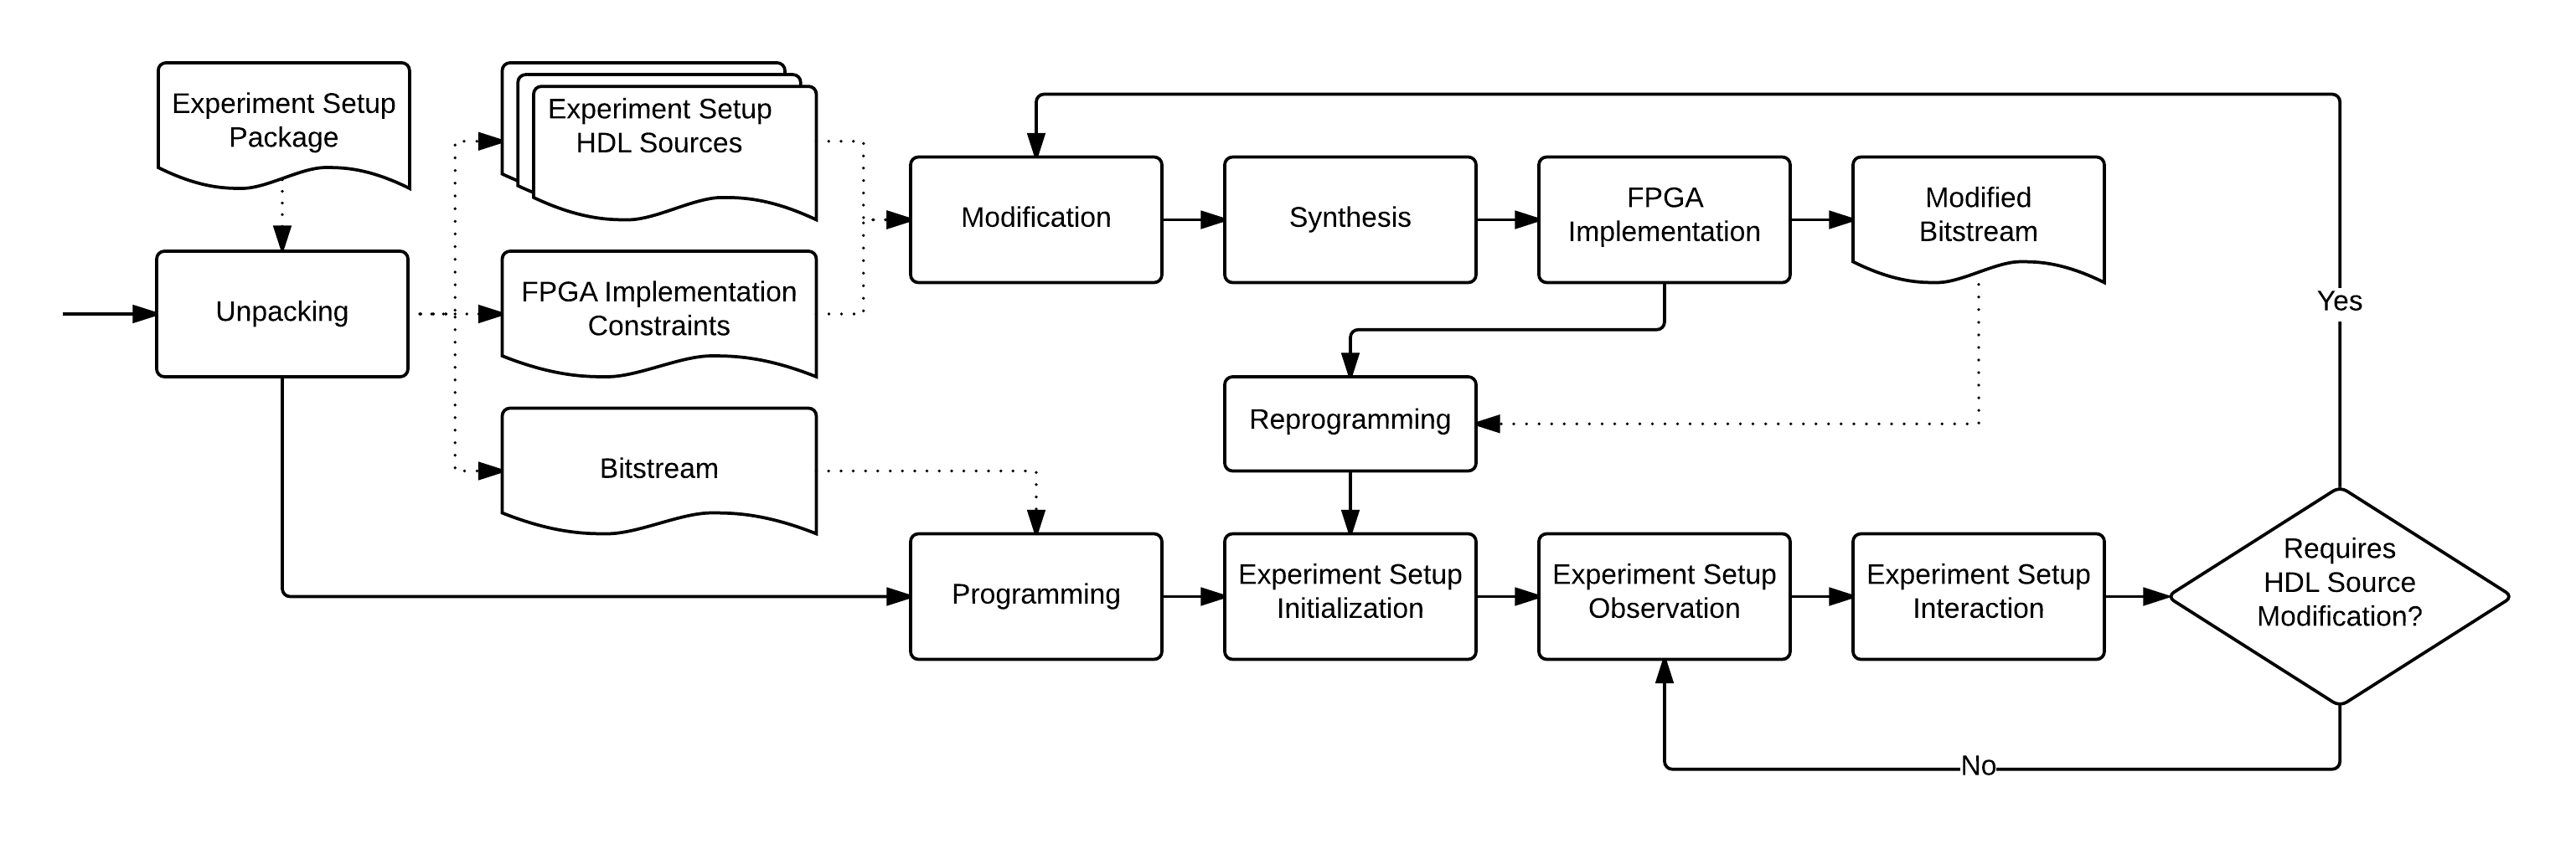
\includegraphics[width=\textwidth]{img/processes-basic-experimentation}
\end{figure}

In order for a user to act as an experimenter, one must understand the logic and workings of the obtained experiment setup. Furthermore, an experimenter must understand the basic concepts and role of the FPGA development board, as well as how to program the FPGA via the experimenter's PC. In preparation of the experiment, experimenters must install programming software and operating system drivers for the FPGA development board. In this case, interaction and observation is done through the board's I/O devices. 

Including the PC as a tool for observation and interaction requires additional knowledge and preparation from experimenters. In order to understand and modify the experiment setup's HDL sources, users must be familiar with the programming language used. Recompilation requires users to install and understand the FPGA's development tools in order to set up a proper development environment. Furthermore, this method of interaction will significantly increase the time required for every change to be processed, since the process of recompilation is a slow process. Using the FPGA as a tool for observation requires further familiarization with the FPGA's development tools.







\section{Virtualizing I/O}
\label{sectionvirtualizingio}

% TODO In deze sectie verduidelijken dat state control nog niet mogelijk is en dat interne state alleen inzichtelijk kan worden gemaakt door expliciet signalen naar buiten te brengen in het experiment ontwerp.

% TODO Er wordt een externe user interface gepresenteerd als oplossing. Hoe ziet deze er uit?

% TODO: Toto: zijn er geen downsides van het gebruik van software?

Regular FPGA development boards offer a limited set of I/O devices. As a consequence, this allows for observation and control of experiment setup logic entities with a limited number of input and output signals. Embedding entities with a large number of inputs and outputs however, requires a different approach. 

In order to support experiment setup entities with a large number of input and output signals, the basic model's logic architecture is extended through introduction of the controller. Figure \ref{fig:fpga-inout} gives an overview of the FPGA and the newly defined architecture. The experiment setup entity's inputs and output signals are available to the controller only, but both components still share a common clock signal. The signal levels of the FPGA's peripheral devices are no longer driven by the experiment setup entity. Following the previous section's criteria, these devices are considered irrelevant and thus removed from the model. Only the clock generating device and a single machine-machine communication device remain part of the model. 


\begin{figure}[h]
\centering
\caption{I/O virtualized, an overview of the FPGA and its contained logic architecture. The controller embeds the experiment setup logic into the FPGA.}
\label{fig:fpga-inout}
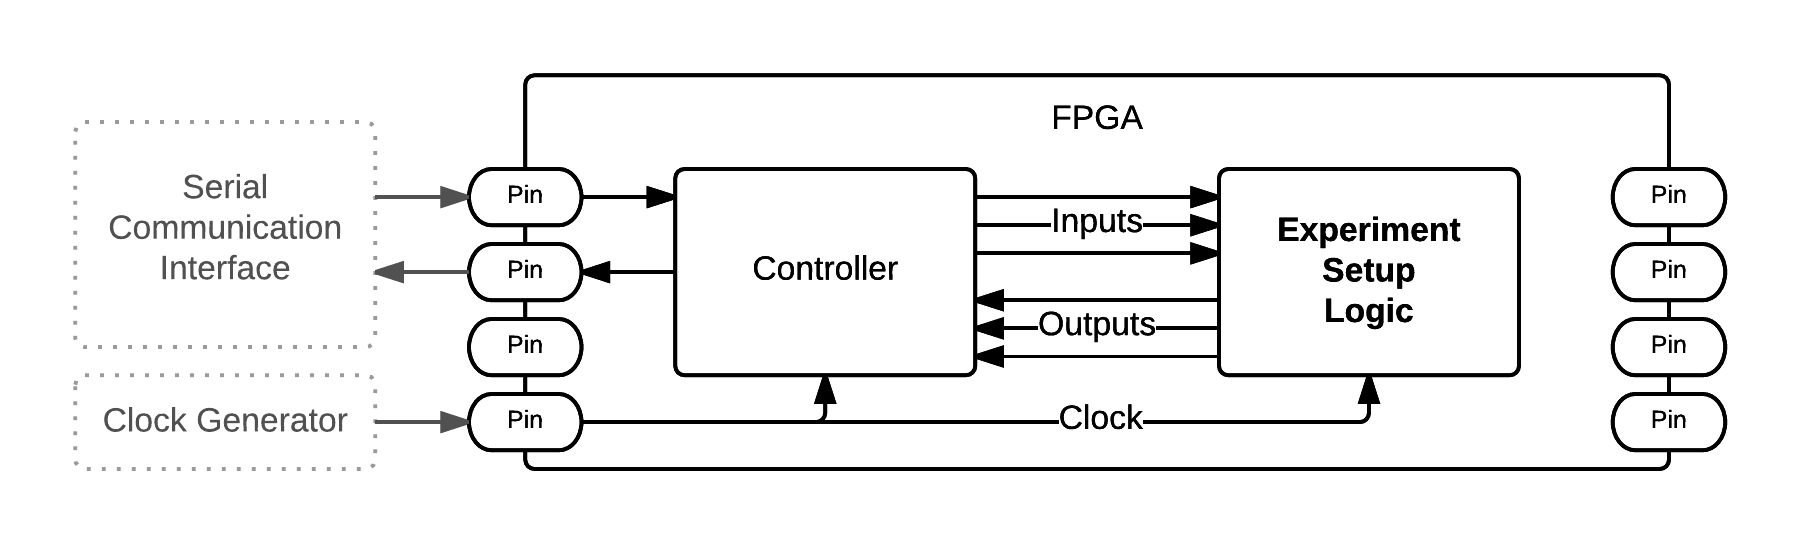
\includegraphics[width=\textwidth]{img/fpga-inout}
\end{figure}

% Concept controller ook te zien in \cite{jansen2014every}

The controller is a component that acts as an intermediary between the experiment setup logic and an experimenter's PC. The experiment setup's state is observed and controlled through controller-specific software, a method also presented in \cite{holland2003harnessing} and \cite{bulic2013fpga}. A hardware-based method to observe and control the experiment setup's state is described in \cite{al2007teaching}. A software-based solution however, does not increase the cost of the experiment. Furthermore, a software-based approach will allow for more flexibility, as shown in the following sections. 

The controller exposes an additional interface through a communication channel that must be provided by one of the FPGA development board's communication devices, as can be seen in figure \ref{fig:overview-inout}. This interface defines operations that allow for the experiment setup entity's individual input and output signals to be controlled and observed respectively. A similar interface for observation and control of specific signals is described in \cite{holland2003harnessing}. 

\begin{figure}[h]
\centering
\caption{I/O virtualized, an overview of the FPGA development board and its exposed interfaces.}
\label{fig:overview-inout}
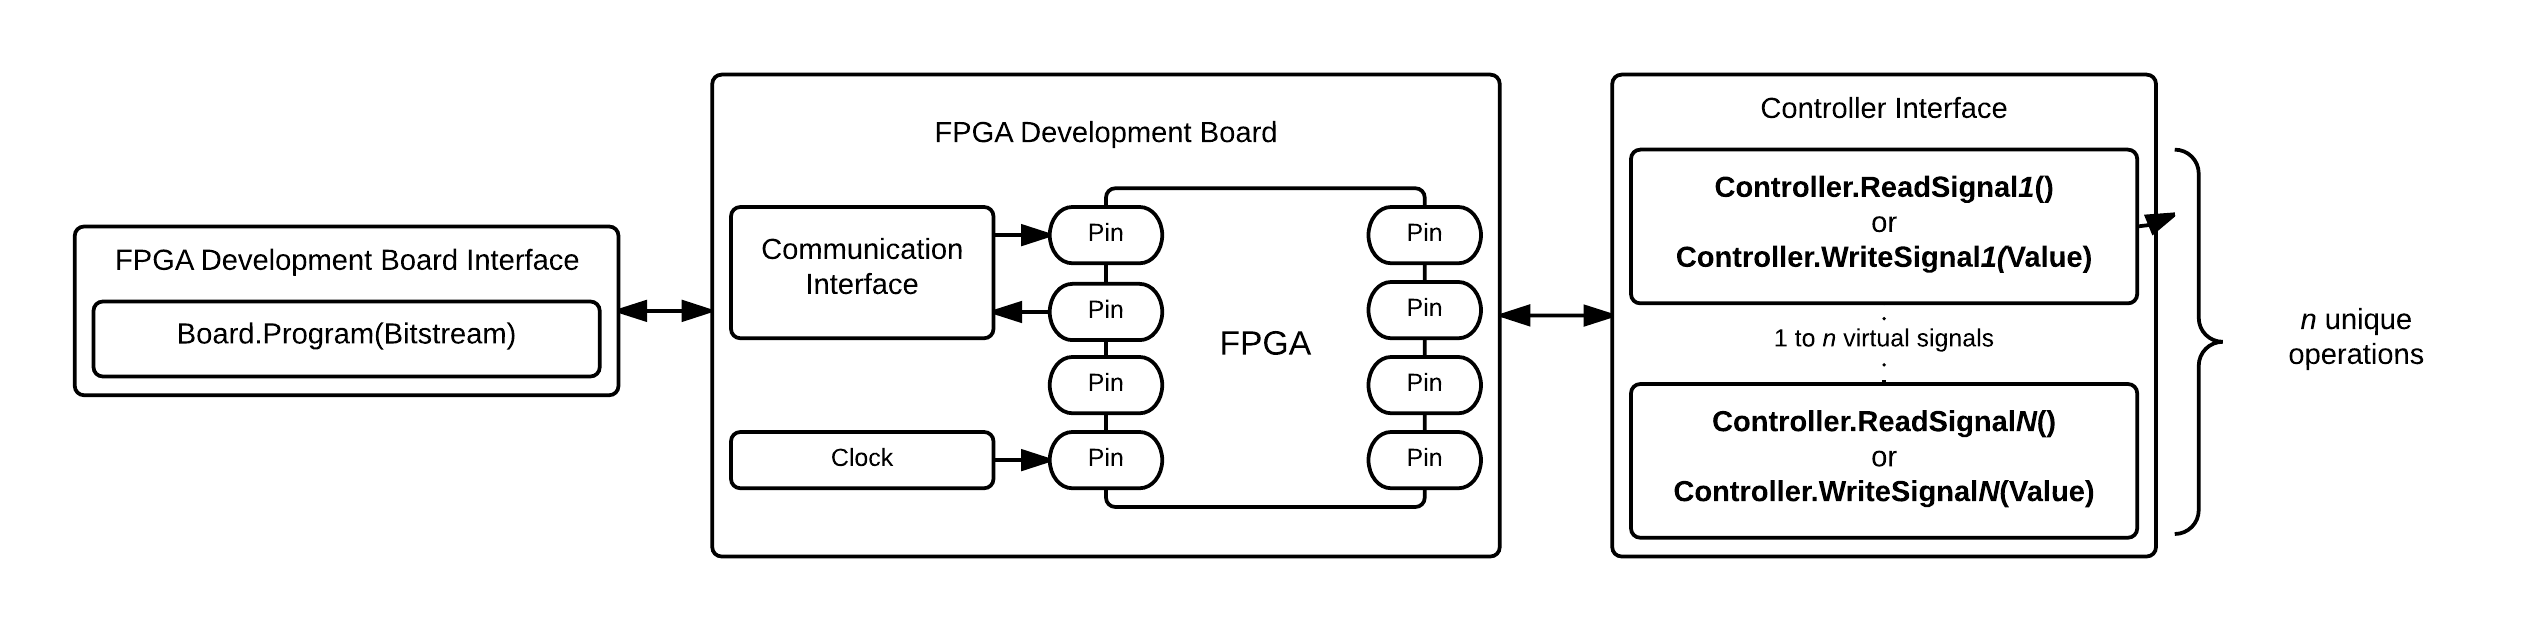
\includegraphics[width=\textwidth]{img/overview-inout}
\end{figure}

The explicit separation of concerns in the logic architecture allows for separate implementation and validation processes for experiment setup logic, controller logic and PC software. This partitioning subsequently allows for distribution of work among specialists, removing the need for a single experiment developer to have knowledge and experience in all the areas previously described in section  \ref{sectionexperimentdevelopers}. As a consequence of the separation however, more dependencies are introduced into the development process. The development of a controller component requires a definition of the experiment setup's interface and any change in this interface definition requires modification of the controller. A similar dependency exists between the controller and the PC software. A change in the experiment setup entity's interface definition will thus not only result in the need for modification of the controller, but in the need for modification of the PC software as well. These dependencies are addressed and removed from the model in section \ref{sectioncontrollerabstraction}.

Experiment setup interaction through dedicated PC software will simplify the experimentation process for experiment setups with large number of input and output signals. Involving the PC removes the need for experimenters to install and familiarize themselves with the FPGA's development tools. Experimenters will be able to interact with the experiment setup through a graphical interface on the PC, removing the need need for HDL programming skills and allowing for real-time interaction, since no recompilation is required. Since the board's I/O devices have been removed at this stage of the model, there is no possibility for users to physically interact with the experiment. The PC software provides the only means of interaction with the experiment setup. These removed I/O devices however, will be reintroduced into the model in section % \ref{sectionreintroducingio}.

% TODO Hoe ziet de PC software er uit?



\section{Cycle control}

% TODO: Taco: Toch eens onderzoeken wat voor mogelijkheden clock domains bieden, mogelijk beschrijven in chapter background.

% TODO: Timing diagram ter verduidelijking clock_enable

\label{sectioncyclecontrol}
In the previous section, the basic model has been extended to include a definition of the controller. This controller allows for the embedding of experiment setup entities with an arbitrary number of input and output signals that are defined through combinational logic. FPGAs in general lack practically useful support for containment of asynchronous sequential logic, but the availability of a clock signal in the current model does provide support for experiment setup entities that are defined through synchronous sequential logic. However, this clock signal is constant and cannot be varied in speed or temporary stopped. Embedding an experiment setup entity of synchronous sequential logic at this stage of the model would result in an uncontrollable situation of continuous state changes at high speed. This limited control over the clock signal is due to the nature of how FPGAs work and prevents cycle-accurate interaction with the experiment setup. In order to be capable of cycle-accurate observations and control over synchronous sequential experiment setup logic, the model requires further extension.

\begin{figure}[h]
\centering
\caption{Cycle control, an overview of the FPGA and its contained logic architecture. The \texttt{clock\_enable} and \texttt{reset} signals are added to allow for cycle-accurate interaction and (re)initialization.}
\label{fig:fpga-control}
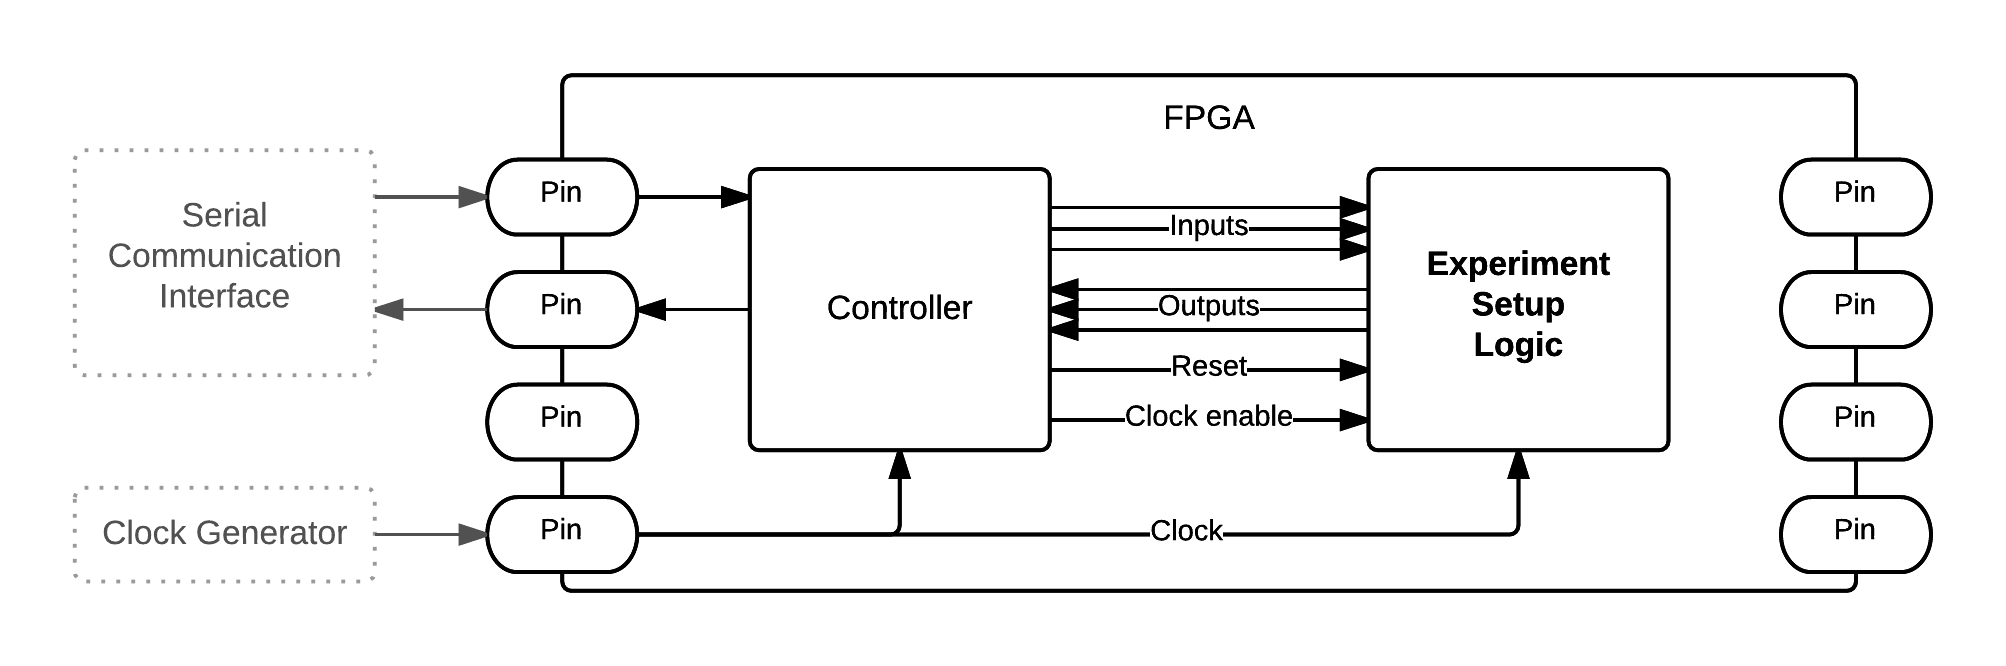
\includegraphics[width=\textwidth]{img/fpga-control}
\end{figure}

As a solution to the problem stated above, the FPGA's contained logic architecture has been extended, as displayed in figure \ref{fig:fpga-control}. The most significant change is the addition of the \texttt{clock\_enable} input signal on the experiment setup's interface definition. Combined with the \texttt{reset} signal, these new input signals allow for cycle-accurate control and reinitialization of the experiment setup logic's state. The introduction of the \texttt{clock\_enable} signal will require modification of every synchronous memory element present in the experiment setup logic, as displayed in figure \ref{fig:clock-manipulation-enable}. By multiplexing the input signal for every memory element based on the same \texttt{clock\_enable}, one can control the state change in a cycle-accurate manner. The method of using enable signals to control synchronous logic is described in \cite[Sec 2.4.5]{arora2011art}.

One may argue that this approach is unfavourable, since it requires modification of existing experiment setup logic designs. This method for controlling state change however, is a common approach in FPGA-targeted HDL development and is used in many designs. More specifically, this approach was also taken in controlling the experiment setups described in \cite{holland2003harnessing} and \cite{bulic2013fpga}. As stated before, FPGAs do not allow for dynamic manipulation of clock signals by design, a method known as clock gating (figure \ref{fig:clock-manipulation-gated} ). Clock signals are distributed over the FPGA through dedicated lines that cannot be altered through HDL logic. Some manufacturers include support for static clock division, but still only down to relatively high speeds and do not allow for dynamic adjustment of clock speed [TODO: Bron]. 

% TODO: Opmerking Taco 
% Opmerking bij fig 3.8 discussie. Het board dat je gebruikt is een artix7
% en die familie (d.w.z. de "7" familie van xilinx) gedraagt zich anders. Er kunnen verschillende clockdomeinen gebruikt worden en dan
% heb je wel degelijk een soort van gated clock, hoewel dat nooit gebeurt via clk_gated = clk_org &
% enable. Lees het 7 series fpga clocking resources user guide document van xilinx!

% TODO: Toto: Meer uitleg bij deze figuren

\begin{figure}[h]
    \centering
    \caption{Controlling state transitions through a clock enable signal and a gated clock signal.}
    \label{fig:clock-manipulation}
    \begin{subfigure}[t]{0.5\textwidth}
        \centering
        \caption{Gated clocks}
        \label{fig:clock-manipulation-gated}
        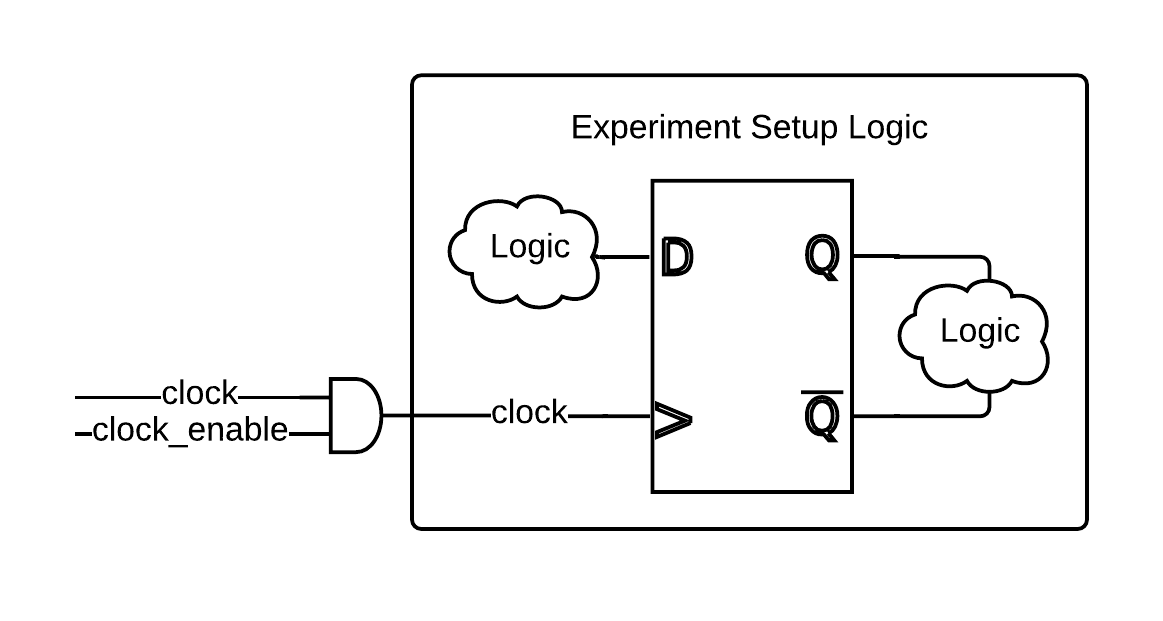
\includegraphics[height=1.5in]{img/clock-manipulation-gated}
    \end{subfigure}%
    \begin{subfigure}[t]{0.5\textwidth}
        \centering
        \caption{Enable signal}
        \label{fig:clock-manipulation-enable}
        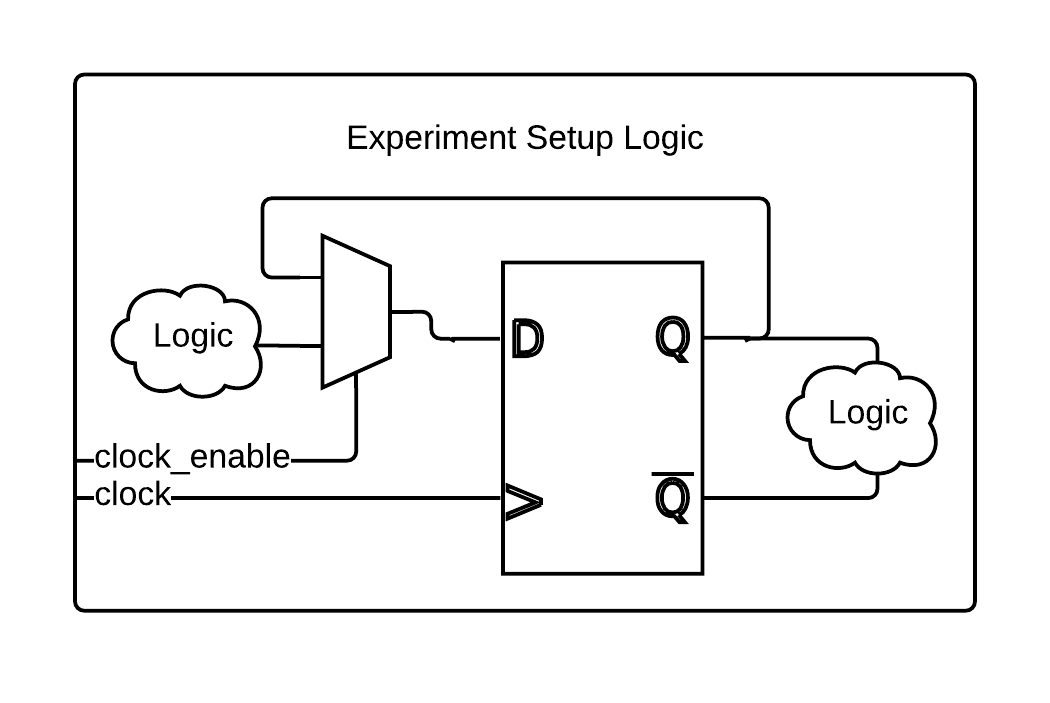
\includegraphics[height=1.5in]{img/clock-manipulation-enable}
    \end{subfigure}%
\end{figure}

In order to make this newly developed functionality available to the experimenter through the PC software, the controller interface is extended to support new operations that allow for the control of cycles. As displayed in figure \ref{fig:overview-control}, five new operations are available through the controller's interface. The \texttt{Controller.Reset()} operation (re)initializes the experiment setup to it initial state and waits for the next operation. Experimenters have manual control over the experiment setup's cycles through the \texttt{Controller.Step()} operation. The controller may also be instructed to manage the experiment setup autonomously through the \texttt{Controller.Start()} operation. The maximum operating frequency may be defined through the \texttt{Controller.LimitSpeed()} operation. The \texttt{Controller.Stop()} operation stops the controller's autonomous management of the experiment setup and awaits the next operation. Similar interfaces for cycle-accurate control of experiment setups are described in \cite{holland2003harnessing} and \cite{bulic2013fpga}.

\begin{figure}[h!]
\centering
\caption{Cycle control, an overview of the FPGA development board. The controller's interface is extended with operations that allow for cycle-accurate interaction with the experiment setup.}
\label{fig:overview-control}
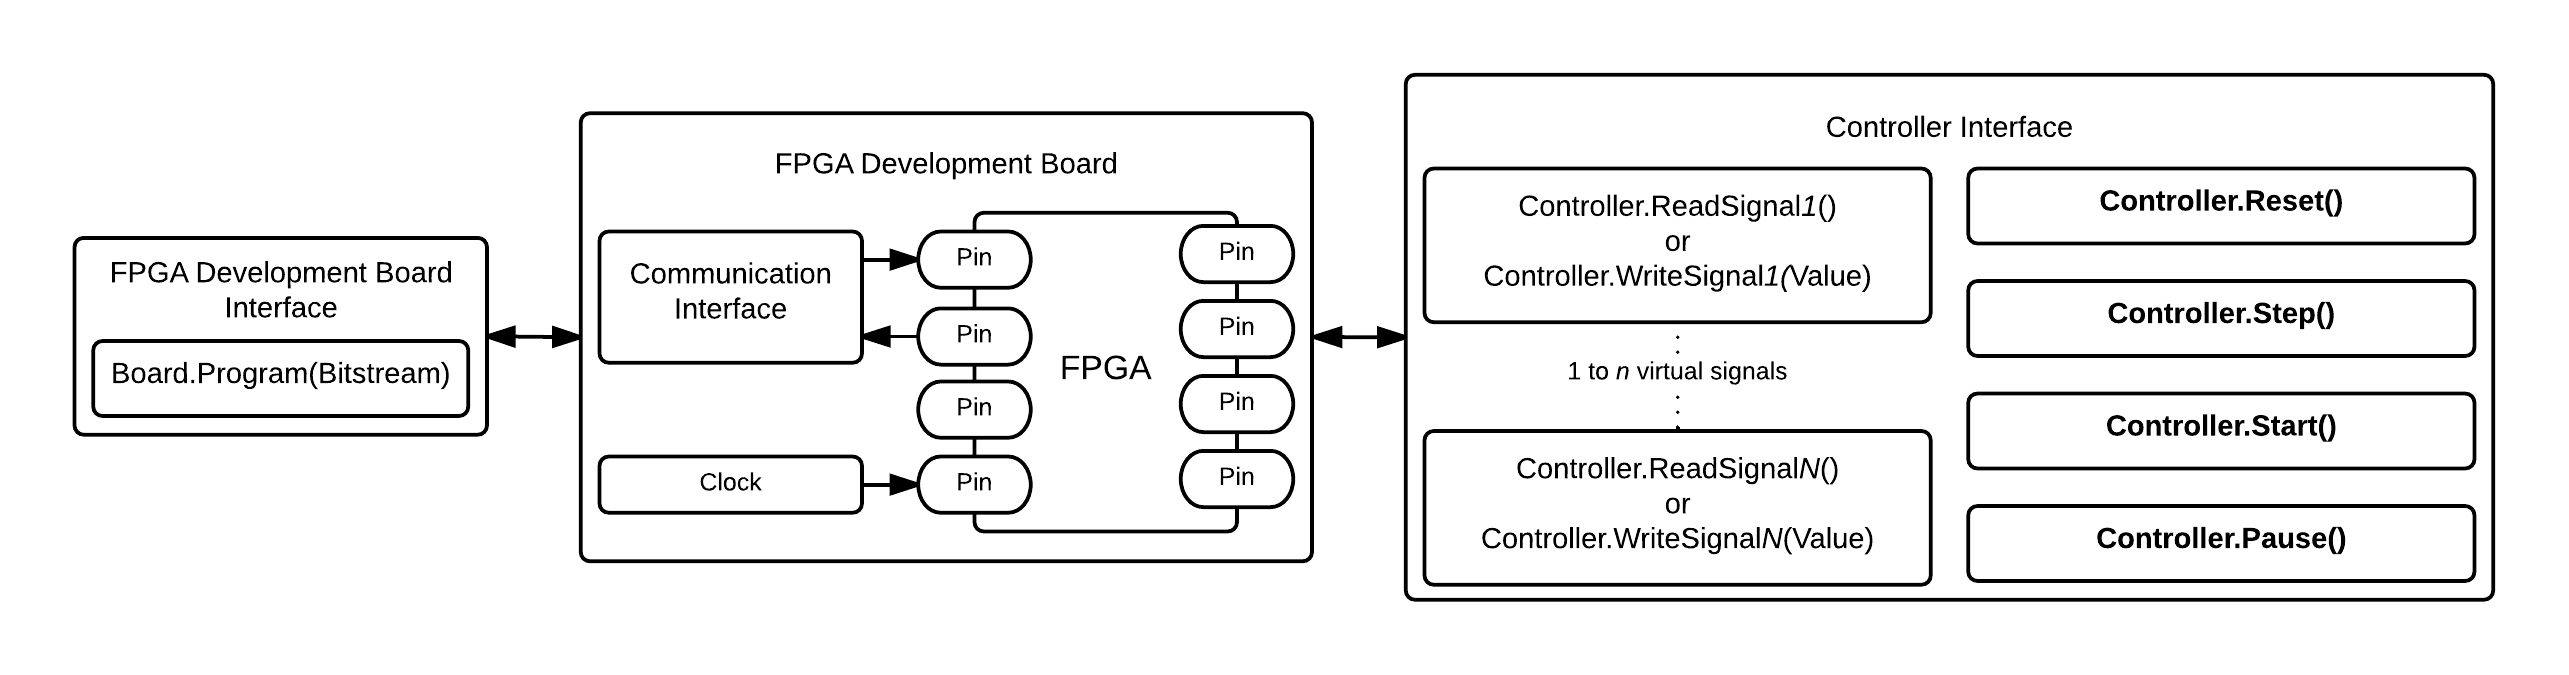
\includegraphics[width=\textwidth]{img/overview-control}
\end{figure}



% TODO: Students must be able to disconnect from the PC and consider the setup as an autonomous entity. The controller interface needs to be extended with a PLAY/PAUSE instruction as well as a means to set the experiment setups clock speed. There needs to be the distinction between a slave mode when connected to the pc as well as a autonomous mode when disconnected.


% \subsection{FPGA Clock management}
% FPGAs generally run on a single clock signal. On modern FPGAs, this clock signal has a frequency in the order of megahertz, which would result in the execution of the experiment at millions discrete steps per second. This clock is generally fixed. In order for students to be able to control their clock speed or even pause their experiment for observations, a second signal must be introduced into the experiment, allowing the enabling of a clock signal. By enabling this 'clock enable' signal for the duration of one clock cycle, the experiment progresses one discrete time step. A disadvantage of this approach is that experiments must be adapted to support this method of managing clocks. This approach however is commonly seen in industry IP components.

% DCM is unsuitable, because it does not allow for halting of the clock signal as well as running on very low frequencies.

% Experiments requiring async clocks can fake this behaviour by deriving a 'clock enable' using a counter.

% See figure \ref{fig:fpga-control}.







\section{Board Component Abstraction}
\label{sectioncontrollerabstraction}

% TODO: Taco: Hoe ga je de inhoud van complexe memory devices inzichtelijk maken?

% TODO: Taco: Wordt de experiment setup adapter gegenereerd?

% TODO: Taco gaat er van uit dat de experiment setup adapter de top component is.

% TODO: Taco: Uiteindelijke functionele omschrijving controller ontbreekt nog

% At this stage of the model's development, it supports the embedding of experiment setups defined through combinational logic as well as synchronous sequential logic. Experimenters can interact with these experiment setups through PC software that is specifically developed for the experiment setup. 
While the model has developed to address a number of problems encountered by experimenters, the problems experienced during development have only been addressed partially. Although an architecture for the FPGA's contained logic was developed in the previous sections, a series of dependencies can still be identified in the development process, as displayed in figure \ref{fig:dependencies-control}.  

The source of these dependencies is the interface between controller and experiment setup. This interface is specific for every experiment setup. By defining a standard interface between experiment setup and controller, this dependency is removed. In the current approach, the experiment setup is considered an entity with inputs and outputs, supplemented by a clock signal, a clock\_enable signal and a reset signal. 

\subsection{Address Space}
%TODO zinnen verbeteren, nog redelijk vaag
% TODO waarom is de keuze voor het model van een address space een goede keuze?
In order to be able to provide a generic interface between controller and experiment setup logic, the experiment setup's interface is modified such that it resembles the interface of a block ram, as can be seen in figure \ref{fig:interface-experiment}. The experiment setup's signals are projected on the address space. 

Losing the information about which signal is which is irrelevant to proper operation of the controller. In order for the PC software to be of any practical use however, a definition of this memory space is required, such that the individual signals can be identified from the memory space. 

The controller does no longer provide an interface to the experiment setup, but acts as a proxy to control the experiment setup's interface. This does not only allow for a reuse of controlling logic, but a simplification as well, since the interface that is exposed to the controller is simplified as well.

\subsection{Interface}
% TODO waarom is een BRAM interface een goede keuze?
%  - eenvoud
% TODO wat zijn de verschillen/voordelen/nadelen t.o.v. andere businterfaces zoals wishbone, AXI etc.
% - wishbone zou een goede optie kunnen zijn ivm open source
% - hoge leercurve bus interfaces
% - master slave interface is voldoende
% - bus interfaces zijn vaak nodeloos complex
% - begrip interface is wijdversprijd
% - ik had niet de capaciteiten om uitgebreid de mogelijke aanvullende voordelen van een businterface te bestuderen, terwijl deze interface voldoende biedt.



\begin{figure}[h]
    \centering
    \caption{Interfaces}
    \label{fig:interfaces}
    \begin{subfigure}[t]{0.5\textwidth}
        \centering
        \caption{Single-port block ram, derived from \cite[Ch.1]{ug473}}
        \label{fig:interface-bram}
        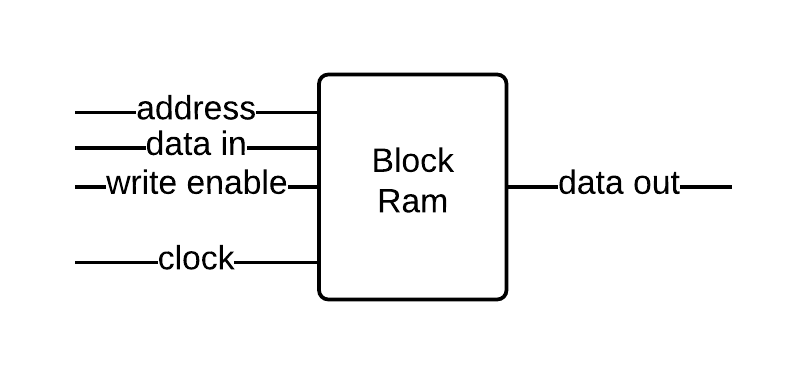
\includegraphics[height=1.2in]{img/interface-bram}
    \end{subfigure}%
    \begin{subfigure}[t]{0.5\textwidth}
        \centering
        \caption{Experiment setup interface}
        \label{fig:interface-experiment}
        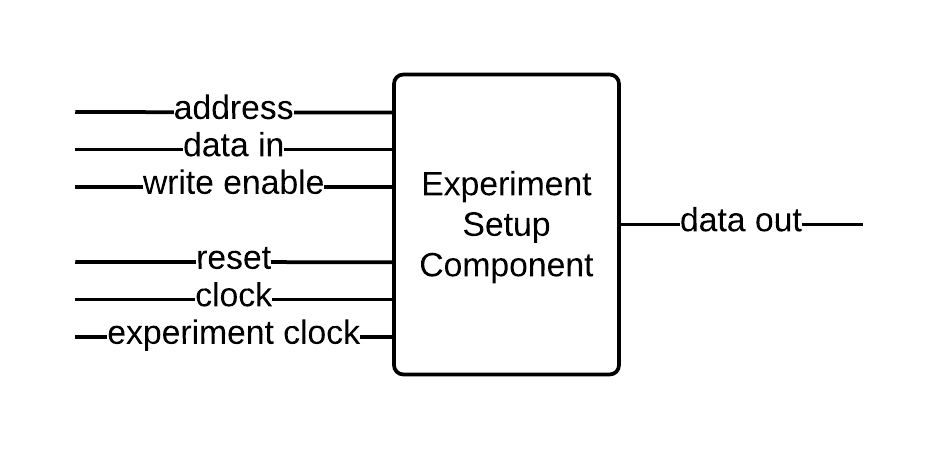
\includegraphics[height=1.5in]{img/interface-experiment}
    \end{subfigure}
\end{figure}

\begin{figure}[h]
    \caption{Timing diagram for experiment setup logic, derived from \cite[Fig.1-2]{ug473}}
    \label{fig:timing-bram}
    \centering
    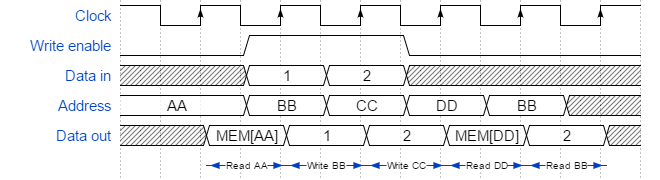
\includegraphics[width=\textwidth]{img/timing-bram}
\end{figure}

\subsection{Memory devices}
%TODO sectie verbeteren, nog erg vage zinnen.

The experiment setup has been considered to be an entity with input output signals. Any memory elements contained within the experiment setup can be made accessible through these input and output signals. This solution is not very scalable however. In order to allow for the controller to read and write to large memory elements such as block rams and register files, a different solution is required. A solution to this problem is displayed in figure \ref{fig:logic-wrap-extended}. 

A simple wrapper can be computer-generated in many cases. If complex memory devices are contained within the experiment setup, a wrapper can be defined manually, using an experiment setup adapter component, address space splitters and memory interface multiplexers. 

Large memory elements such as register files and block rams may be defined in HDL. During the compilation process, these elements are infered from HDL code and the FPGA's internal block rams are used. 

% If more memory space is required however, external memory devices such as DDR RAM IC's may be required. Since these external RAM devices require a number of cycles in order to accress the data, they must be abstracted in order to be accessible from within the experiment setup logic. In order to achieve the desired effect of seeing these DDR RAM devices as block ram devices that only require a single clock cycle to operate, the controller must stall the \texttt{clock\_enable} signal until the DDR controller finishes the desired operation. 


\subsection{Composition Process}
In stead of the distinction between controller and experiment setup, a new separation is defined in the controller's logic architecture. A distinction is made between the logic that is targeted to a specific FPGA development board and the logic that targets the standard board component interface. Figure \ref{fig:fpga-abstract} displays this distinction. This distinction is made, because the experiment setup is no longer being defined by it's primary logic, but as secondary interfacing logic as well. 

% The controller was defined to be a specific implementation embedding a specific experiment setup into a FPGA development board.

\begin{figure}[h]
\centering
\caption{Controller abstracted, FPGA logic design}
\label{fig:fpga-abstract}
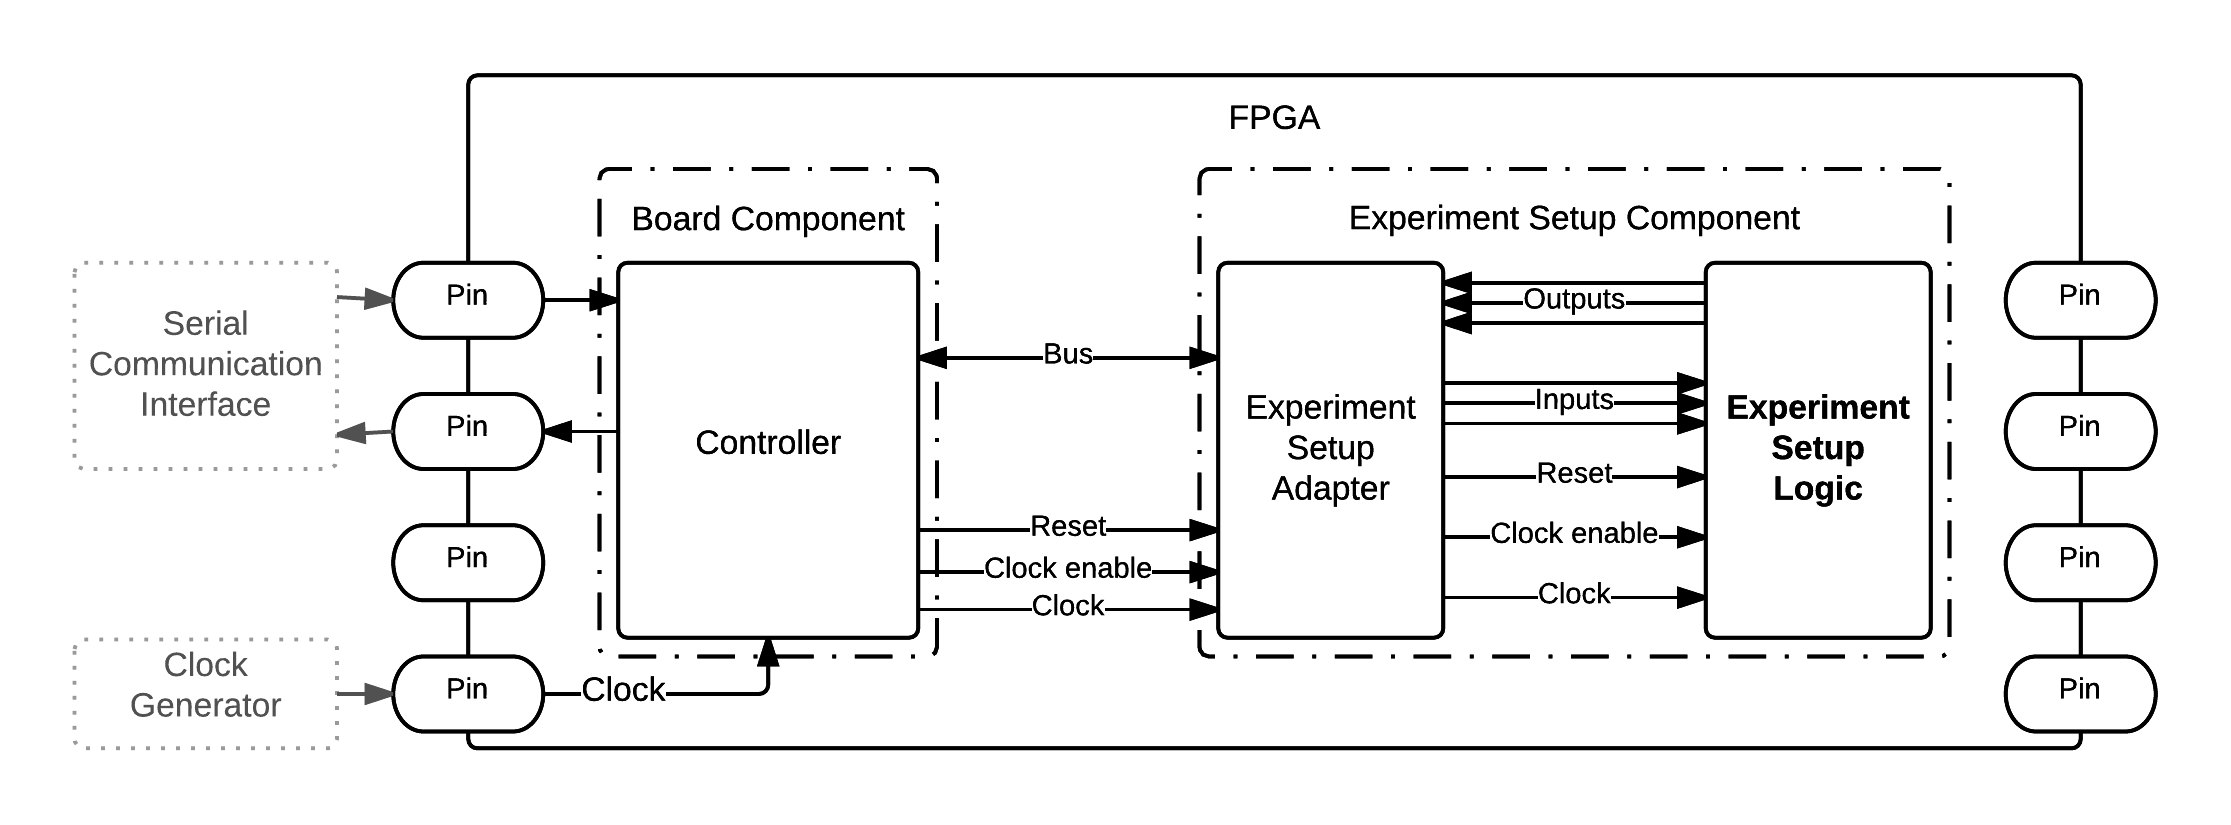
\includegraphics[width=.8\textwidth]{img/fpga-abstract}
\end{figure}

A new process is defined for the composition of board component and experiment setup component into a bitstream file. This results in the processes of experiment setup development and board component development to become independent. Figure \ref{fig:dependencies-abstract} displays the composition process and its relation to the  development processes for experiment setup component and board development component in terms of dependencies. 

\subsection{Experiment Setup Adapter}

In order for an experiment setup logic to conform to the experiment setup component's interface, a component is introduced that acts as an adapter. This experiment setup adapter is a logic component that projects the experiment setup's input and output signals onto an address space. Figure \ref{fig:fpga-abstract} displays the experiment setup adapter.




\subsection{Generic PC Software}
A major advantage of the generic interface between the controller and experiment setup is that PC software can be developed that is no longer specifically tied to one particular experiment setup design. The controller now acts as a proxy between the PC and the experiment setup. The experiment setup is considered an address space from the PC software, no longer an entity with inputs and outputs. In order for this address space to be of any significant meaning, the PC software requires information on how the data in this address space is structured. During the wrapping process a file will be generated, describing how the experiment setup's signals are projected onto its address space. 

% iets zeggen over de faciliterende interface tussen PC en 



\begin{figure}[h]
\centering
\caption{Controller abstracted, overview}
\label{fig:overview-abstract}
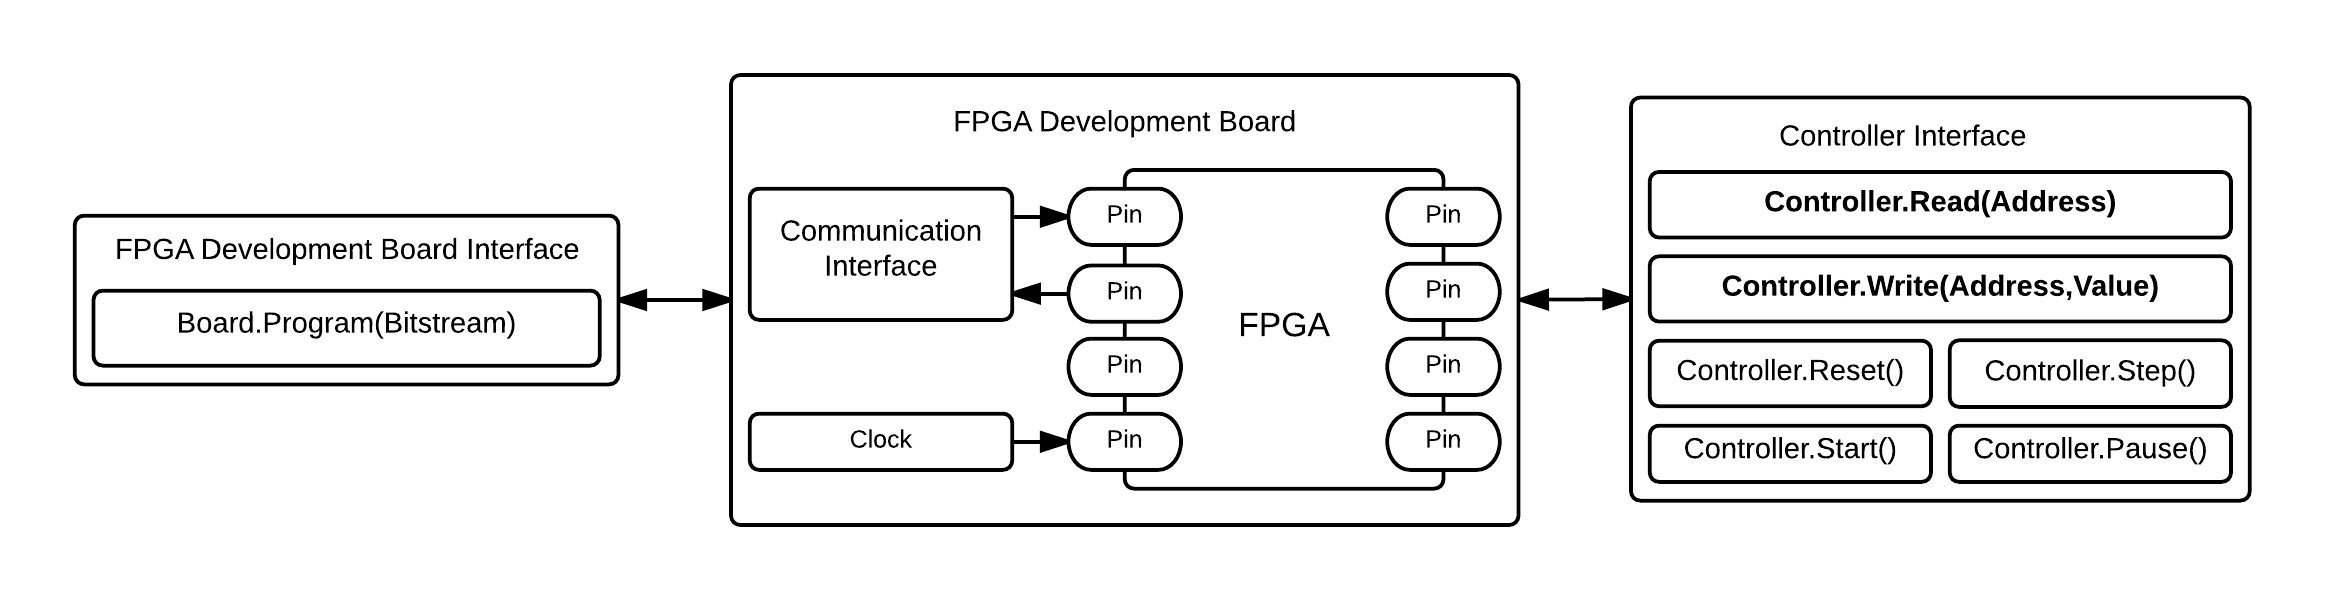
\includegraphics[width=\textwidth]{img/overview-abstract}
\end{figure}


%variable address width
%variable data width

% studenten:
% - nog niet mogelijk snel te switchen
% docenten
% - afhankelijkheden tijdens ontwikkelproces.

% het is nog niet mogelijk te interfacen met complexe state devices in 

% Developed experiment setups are still board-specific

% Software is still controller-specific

% Controller-specific software

% Experiment-specific controller

% abstraction Allows for reuse of code

% abstraction allows for board-independent experiment development

% abstraction allows for random combination of experiment and controller, allowing for reuse of experiment code

% introduction of standard interfaces removes dependencies from development process

% Removing the dependency from controller to experiment, generic interface.

% Allows for reuse of generic board components for different experiment setup components.

% Complicates experiment development, but process of wrapping can be automated

% view of experiment as address space allows for easy interface from software address space allows for projection of signals as well as memory elements.









% \section{Reintroducing Board I/O}
% \label{sectionreintroducingio}

% Experiment setup has no accurate notion of time, so I/O devices can only be addressed as combinational devices. I/O device drivers facilitate this.

% Board I/O capabilities are of vital iportance in providing a physical hands-on experience. Although the FPGA itself is a physical object, the board's I/O capabilities expose the hardware setup's physical behaviour and provide real life interaction capabilities. Without this step, the whole point of a physical hands-on experience is lost.

% See figure \ref{fig:fpga-io}

% \subsection{I/O processing}
% Optionally, one needs to introduce device driver logic in order to allow for sequential I/O device logic to be usable as combinational logic. 




% \begin{figure}[h]
% \centering
% \caption{I/O reintroduced, overview}
% \label{fig:overview-io}
% 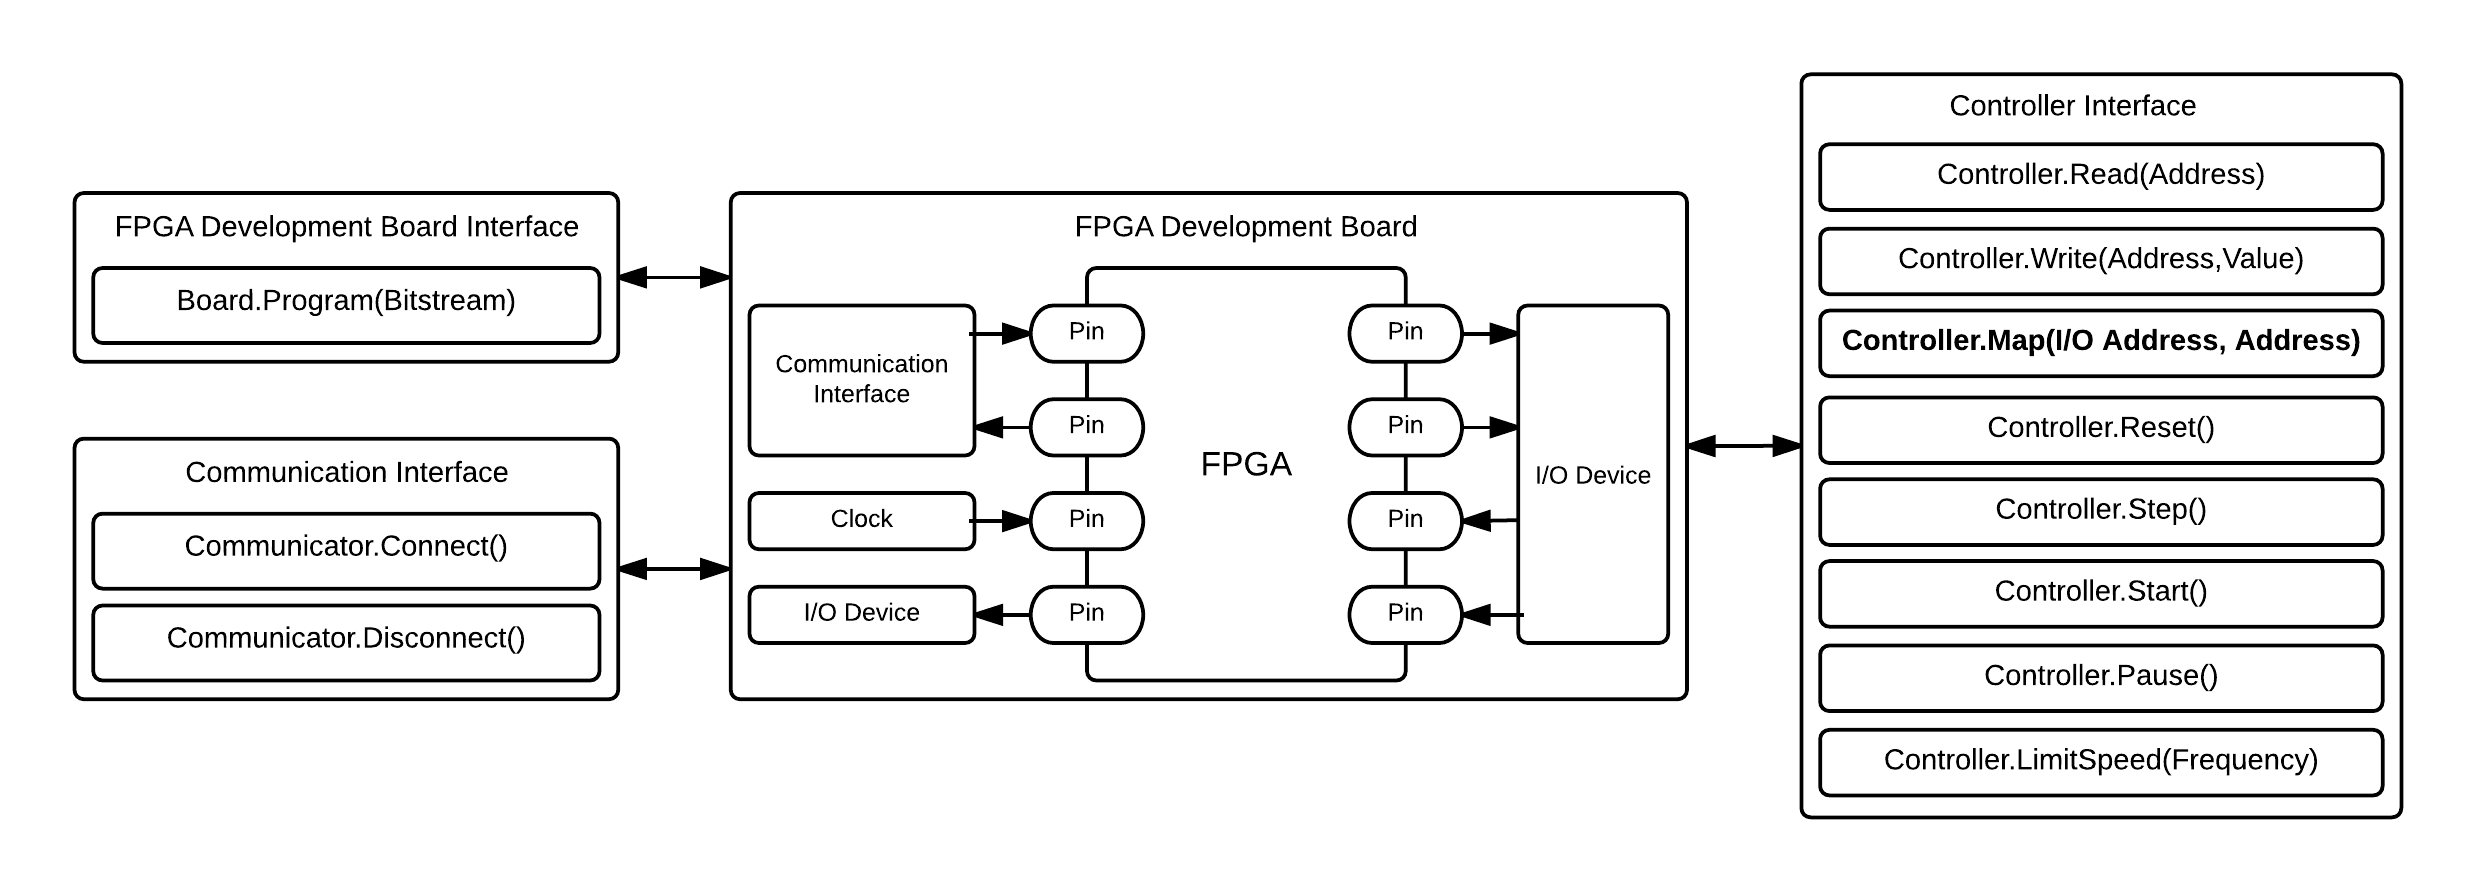
\includegraphics[width=\textwidth]{img/overview-io}
% \end{figure}


% \begin{figure}[h]
% \centering
% \caption{I/O reintroduced, FPGA logic design}
% \label{fig:fpga-io}
% 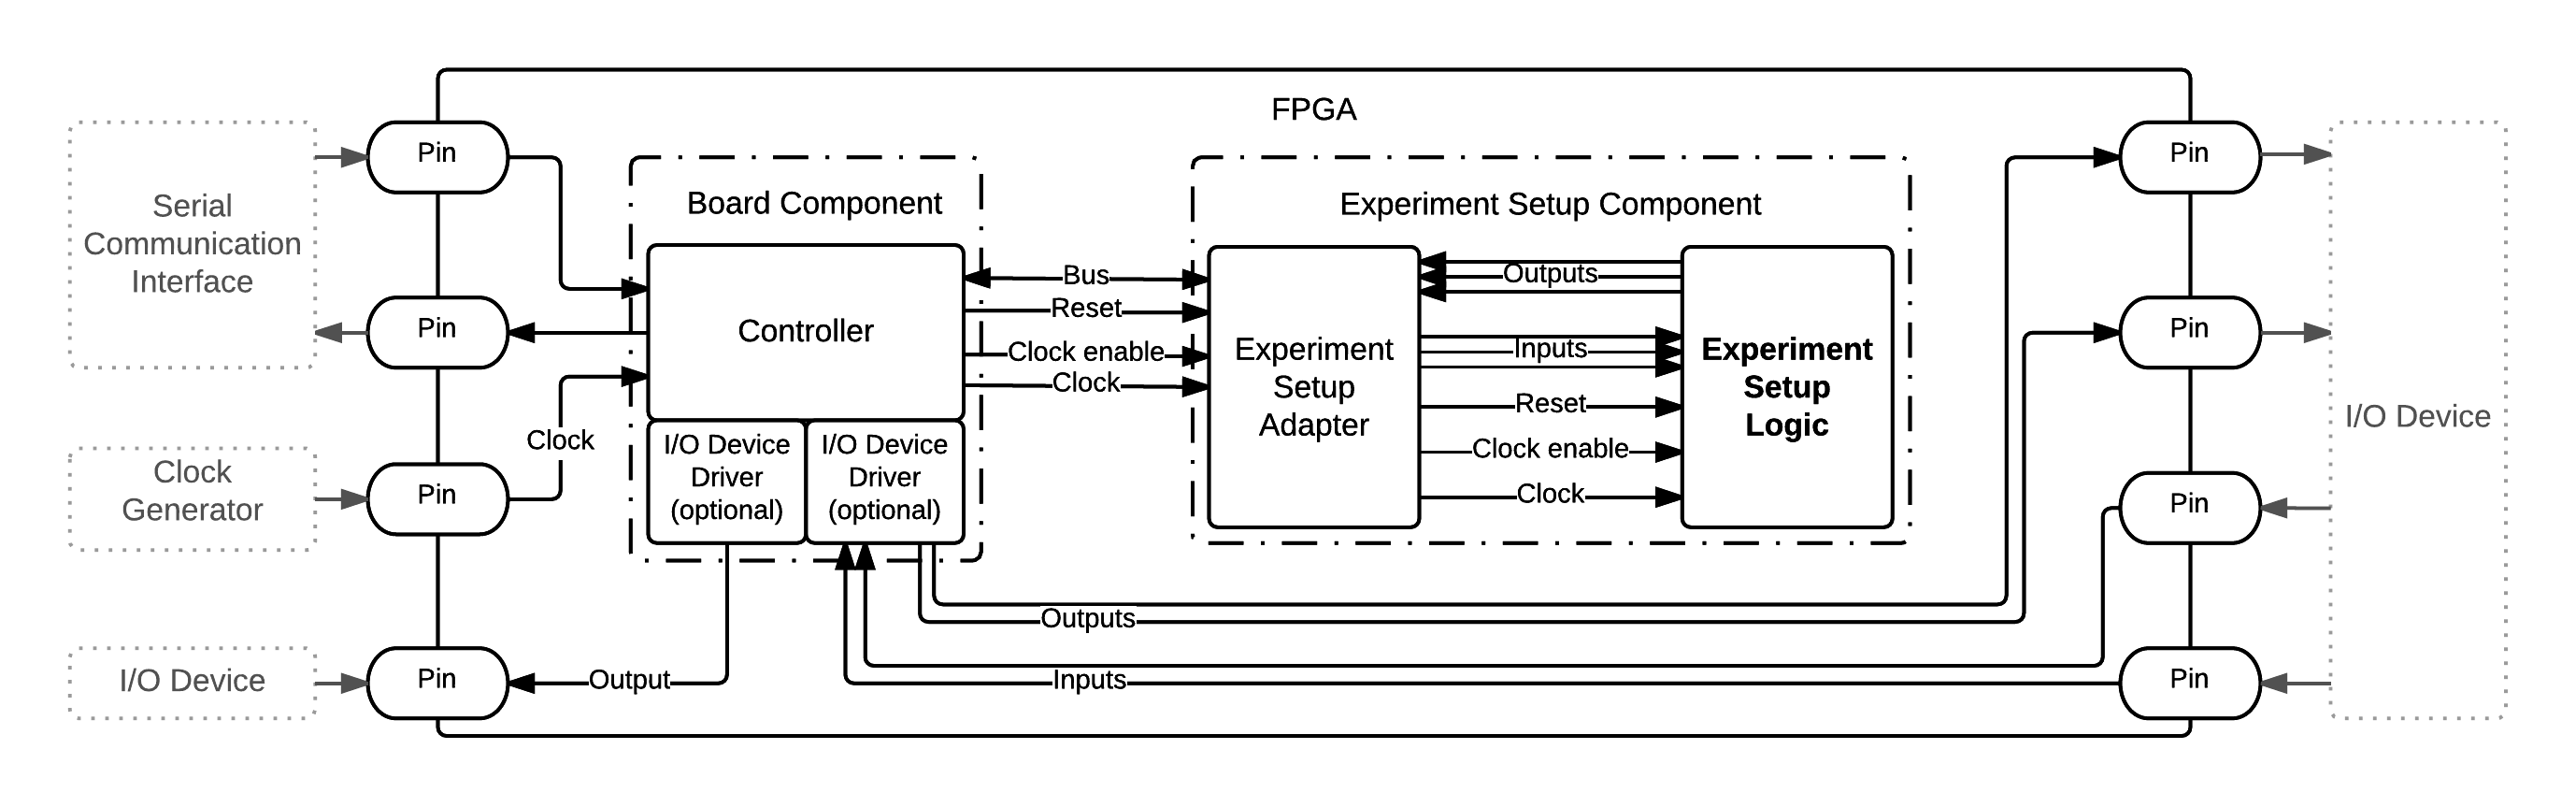
\includegraphics[width=\textwidth]{img/fpga-io2}
% \end{figure}

% \begin{figure}
% \centering
% 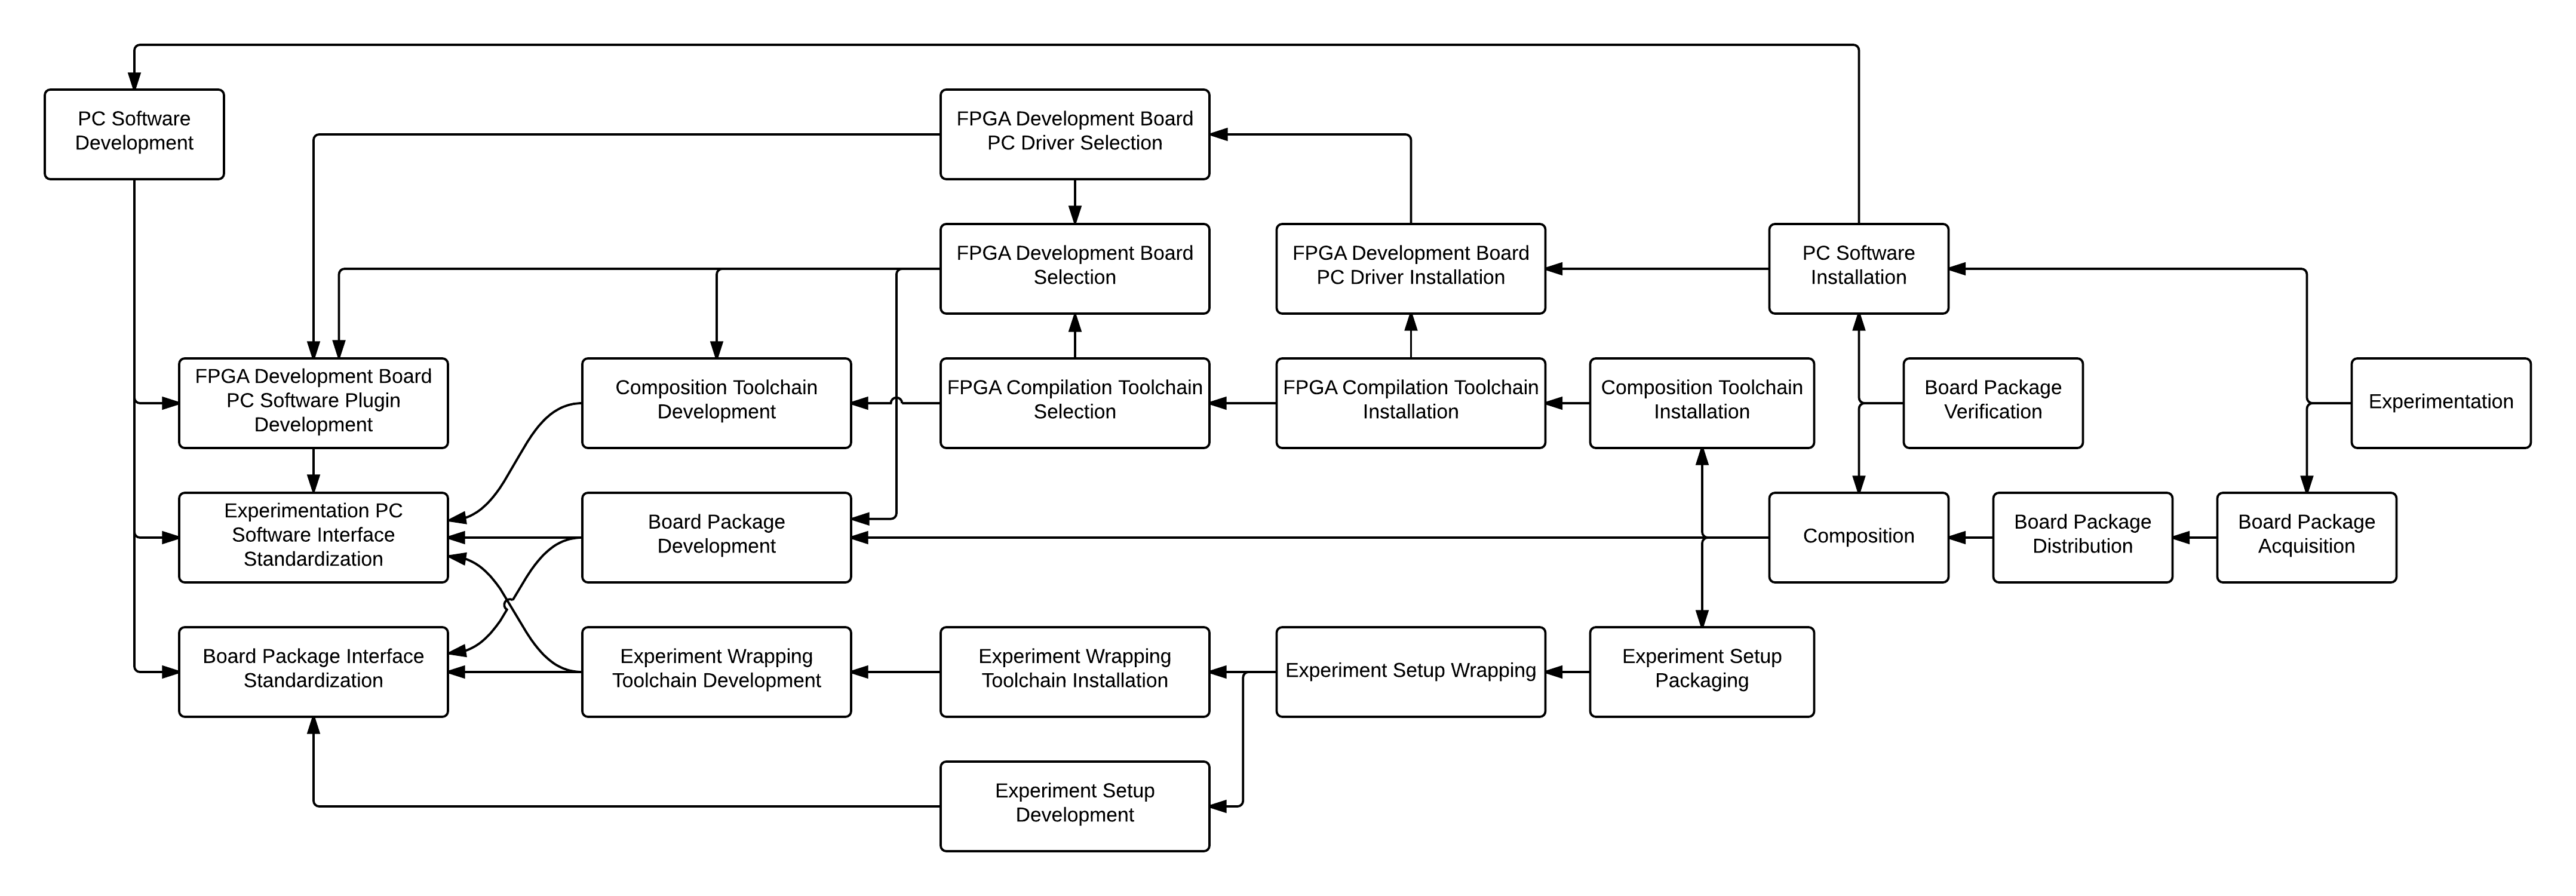
\includegraphics[width=\textwidth]{processes-dependencies-io}
% \caption{I/O reintroduced, Process dependency graph}
% \label{fig:processes-dependencies}
% \end{figure}

% \begin{figure}
% \centering
% \makebox[\textwidth][c]{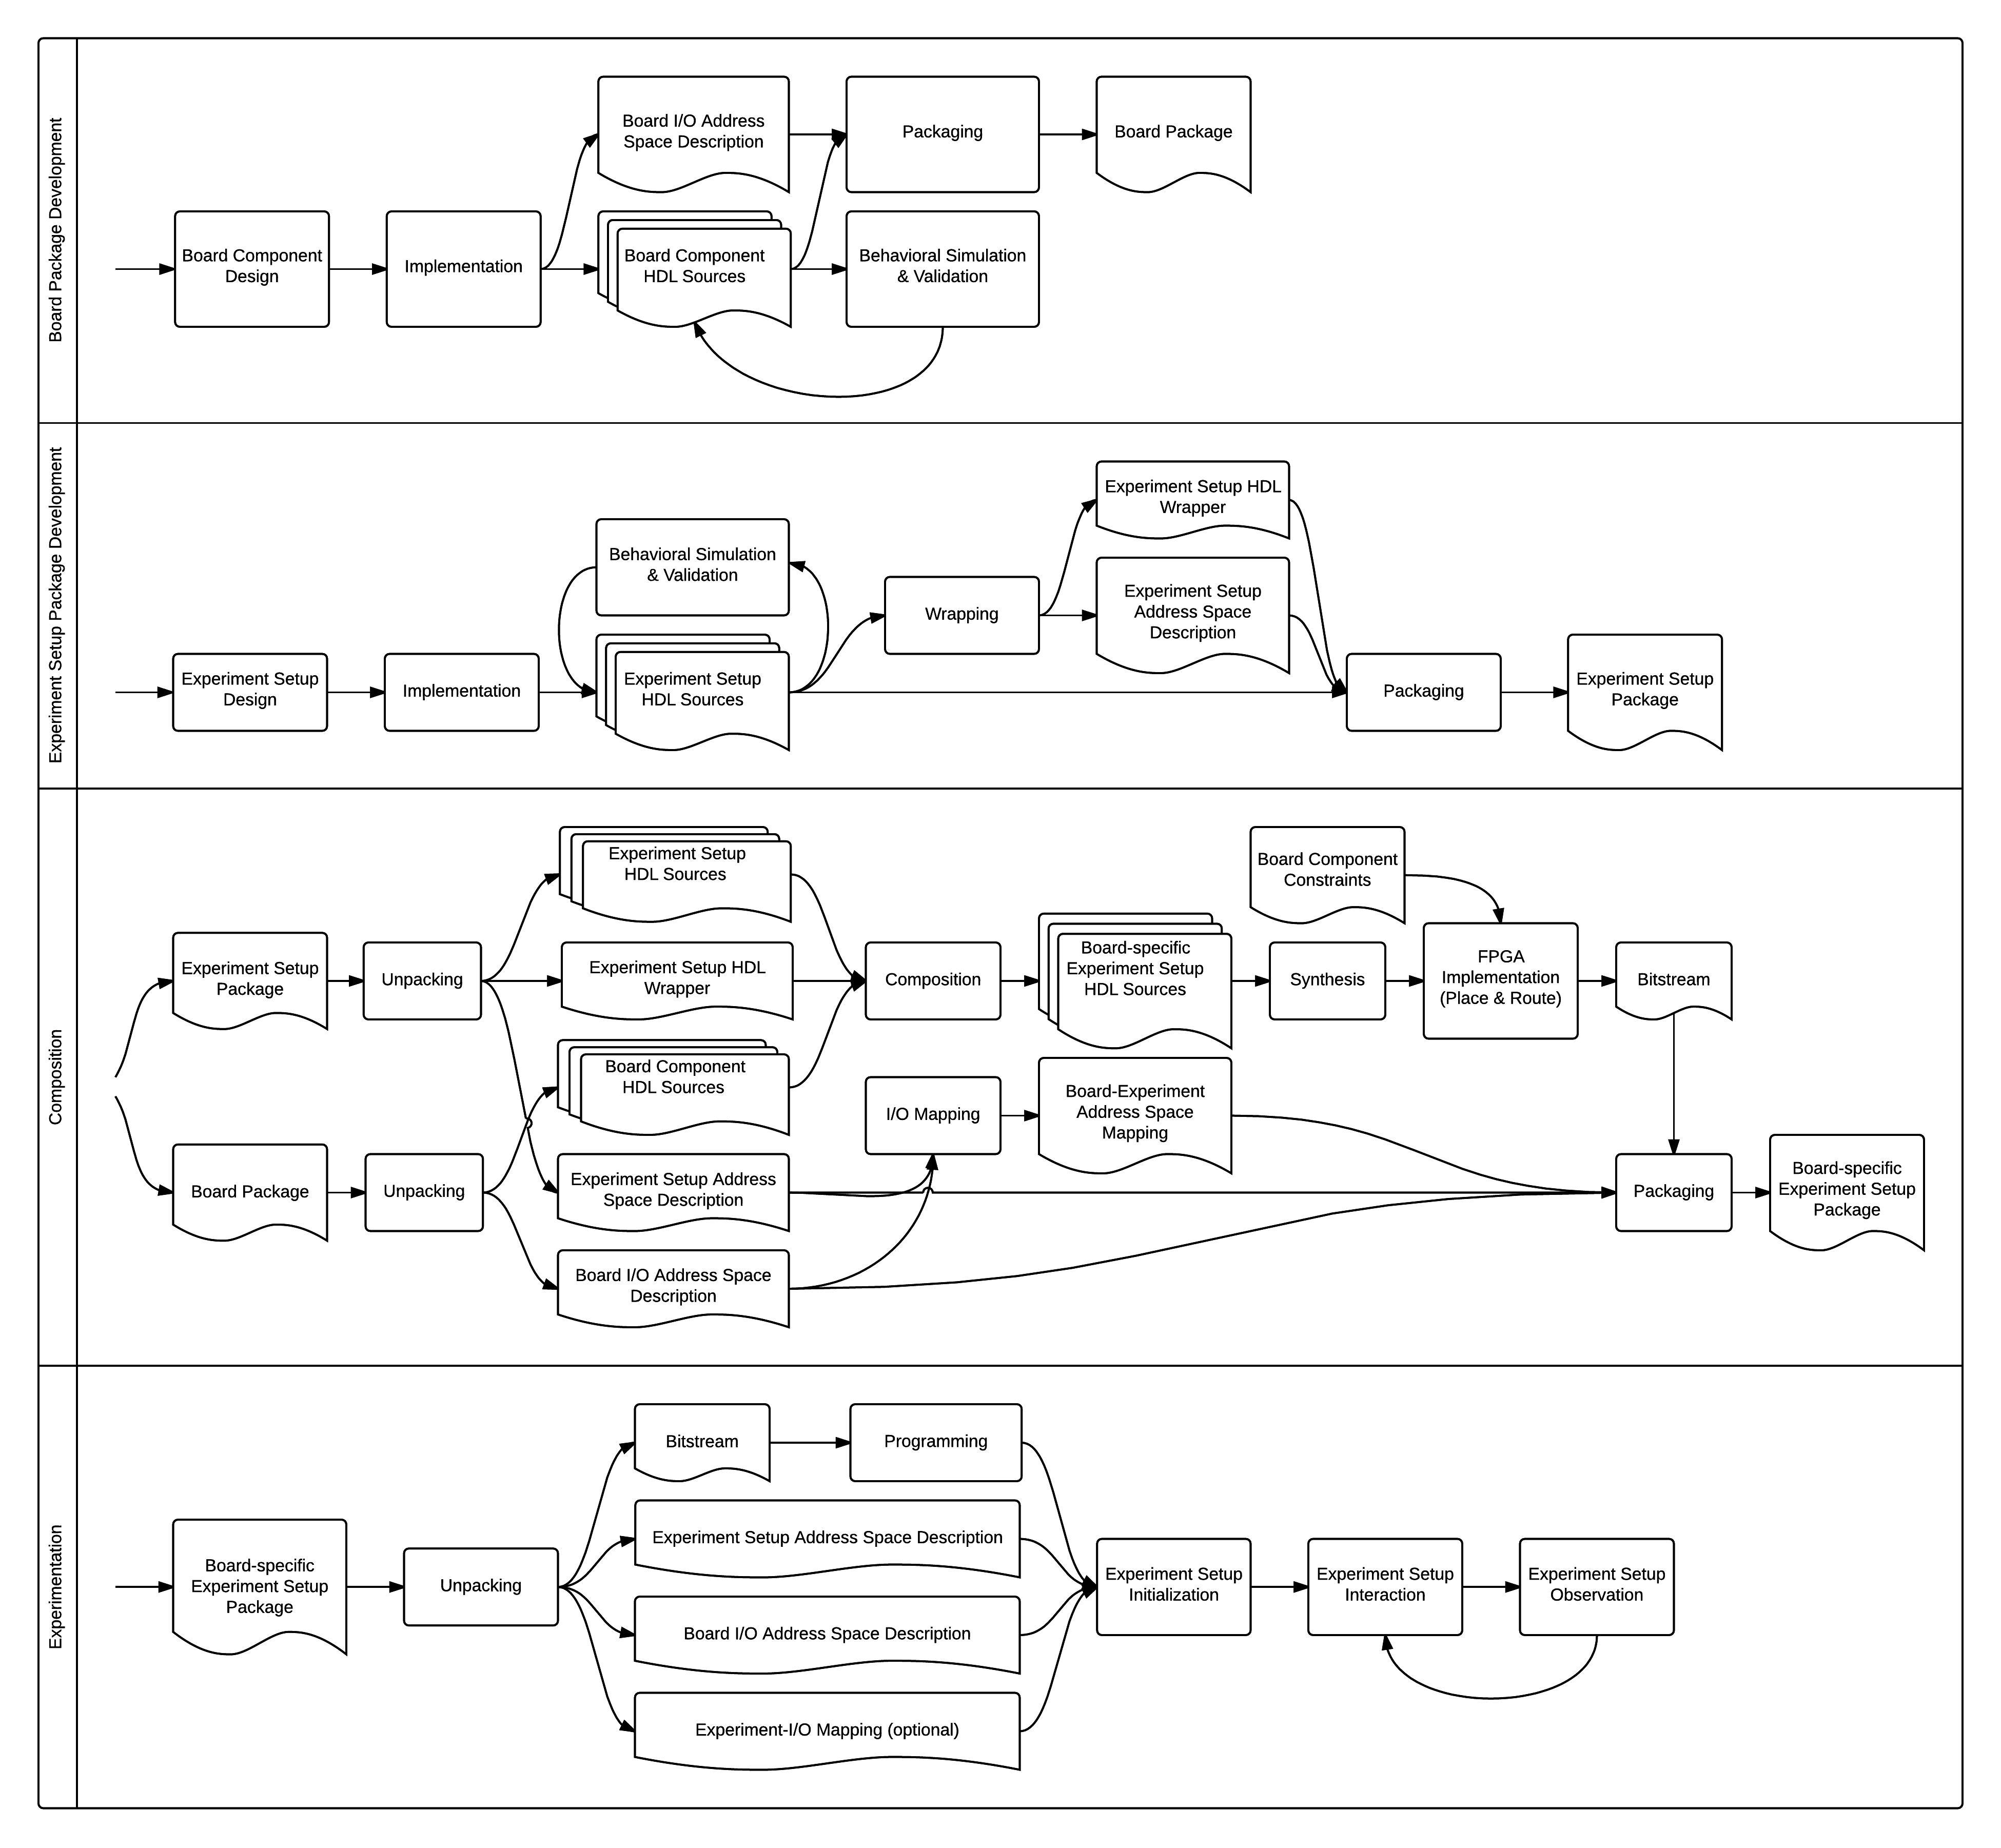
\includegraphics[width=1.25\textwidth]{processes-io}}
% \caption{I/O reintroduced, Processes overview}
% \label{fig:processes-io}
% \end{figure}

% \section{Student Requirements}
% A FPGA development board is connected to a student's PC. Two issues need to be addressed: an easy way of programming the FPGA in order to setup the experiment and communication with the FPGA to allow for interaction during the experiment. 

% Manufacturer development tools often facilitate these functions.

% They install FPGA board operating system drivers and experiment host software. An experiment is prepared by the course instructors and distributed to students. By loading the experiment, the fpga should be automatically programmed. The FPGA is not reprogrammed during the experiment. The student only interacts with the experiment through the experiment host software or the physical board as if it were the experiment hardware itself. 

% \section{Instructor requirements}
% It should be easy for instructors to create, test and distribute experiments. For the development of these experiments, instructors should be able to make use of existing development tools. 

% \section{Conceptual Model}
% In combinatorial logic, the output of signals is not dependent on the state of the digital circuit. In sequential logic, the output is dependent on the input signal levels, as well as the levels of previous input signals, the state of the circuit. Sequential logic is usually synchronous, meaning that state changes are triggered by a clock signal. 

% The circuit's state needs to be transfered to the student's PC such that it can be interpreted. 

% From an abstract point of view, a sequential circuit's state can be seen as a series of signals. Some signals are singular bit values, while others are composed of multiple bit values. Signals can be independent, while similar may be grouped by function, such as a set of cpu registers, data memory or instruction memory. 

% All these signals may be projected onto a memory space in order to allow for all signals of an experiment setup to be represented uniformly. 

% A file combined with the fpga program instructs the PC software on how to the memory space should be interpreted. This file is specific for one single version an FPGA program, but the same accross different FPGA board and desktop tools. In the fpga program it is determined how the experiment's signals are mapped onto the memory space. The PC software interprets these signals. 

% A fpga program may support multiple types of communication, such as serial rs232, ehternet, pci express etc...

% A distributable is specific for a combination of a FPGA development board model, a version of the FPGA program and a version of the PC tools. 

% The pc software must allow for the loading of a distributable, programming the experiment onto the FPGA and establishing a connection such that it can control the experiment. The PC software interprets the memory map of the fpga program and adapts its interface. After establishing a connection, the student can start the experiment by manually stepping a clock cycle, or set the clock cycle to increase automatically at a defined frequency. 


\end{document}